\section{IMPRS-MPA}

%\frame
%{
%%...................................................................................................
%\note<1>[]{}
%%...................................................................................................
%	\frametitle{}
%	\begin{itemize}
%		\item 
%	\end{itemize}
%	\centering
%%	\includegraphics[width=115mm]{images/}
%}


\frame
{
%...................................................................................................
\note<1>[]{}
%...................................................................................................
	\frametitle{First project - Introduction}
	\centering
    \large{\textbf{OODF: Optimized Opacity Distribution Functions for a New Generation of Solar and Stellar Brightness Variability Models}} \\
    Miha Cernetic, Alexander I. Shapiro, Veronika Witzke, Natalia A. Krivova, Sami K. Solanki, \\Rinat V. Tagirov
}

\frame[t]
{
%...................................................................................................
\note<1>[]{Total solar irradiance is defined as spectrally integrated solar radiative flux at 1 AU. It is measured in W/m^2. The plot shows that th TSI varies on timescales from minutes to decades. So what is the main contributor to this variability?}
%...................................................................................................
	\frametitle{\alert{T}otal \alert{S}olar \alert{I}rradiance}
	\begin{itemize}
		\item TSI -- spectrally integrated solar radiative flux at 1 AU from the sun \\
	\end{itemize}

	\centering
	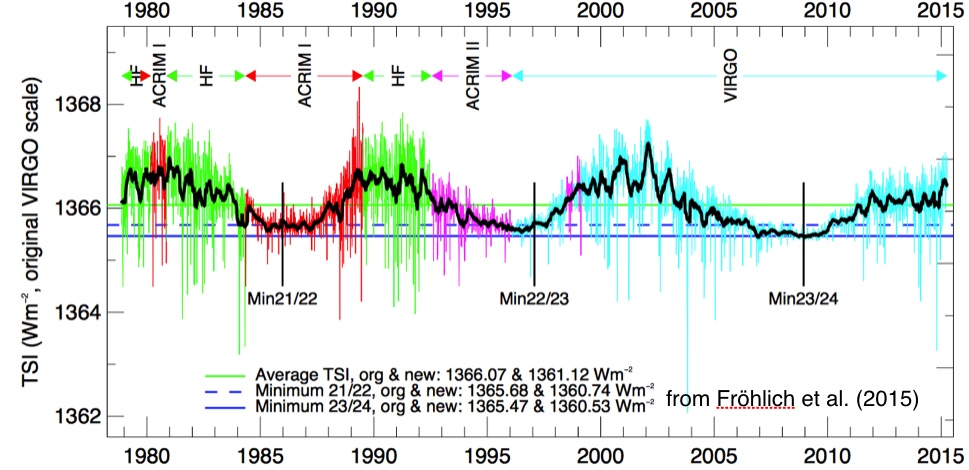
\includegraphics[width=130mm]{images/tsi}
	
}

\frame
{
%...................................................................................................
\note<1>[]{If we want to obtain the emergent spectra from a 3D MHD cube which gives us the structure of the magnetic fields we pierce it with 1k rays and then calculate the emergent spectra from those 1D atmospheres. There are multiple methods how to speedup RT and here is were my work comes in. I will show you my work on ODF and the improvements we have made on them. }
%...................................................................................................
	\frametitle{1.5D simulations}
	\centering
	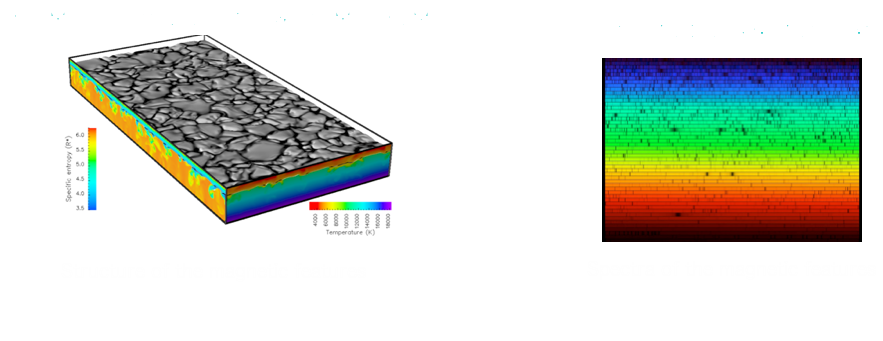
\includegraphics[width=150mm]{images/1_5D}
}

\frame
{
%...................................................................................................
\note<1>[]{If we look at the solar spectra we see that it has very complex structure. It is full of spectral lines.}
%...................................................................................................
	\frametitle{Spectra of the individual components}
	\centering
	\LARGE Observed solar spectra \\
	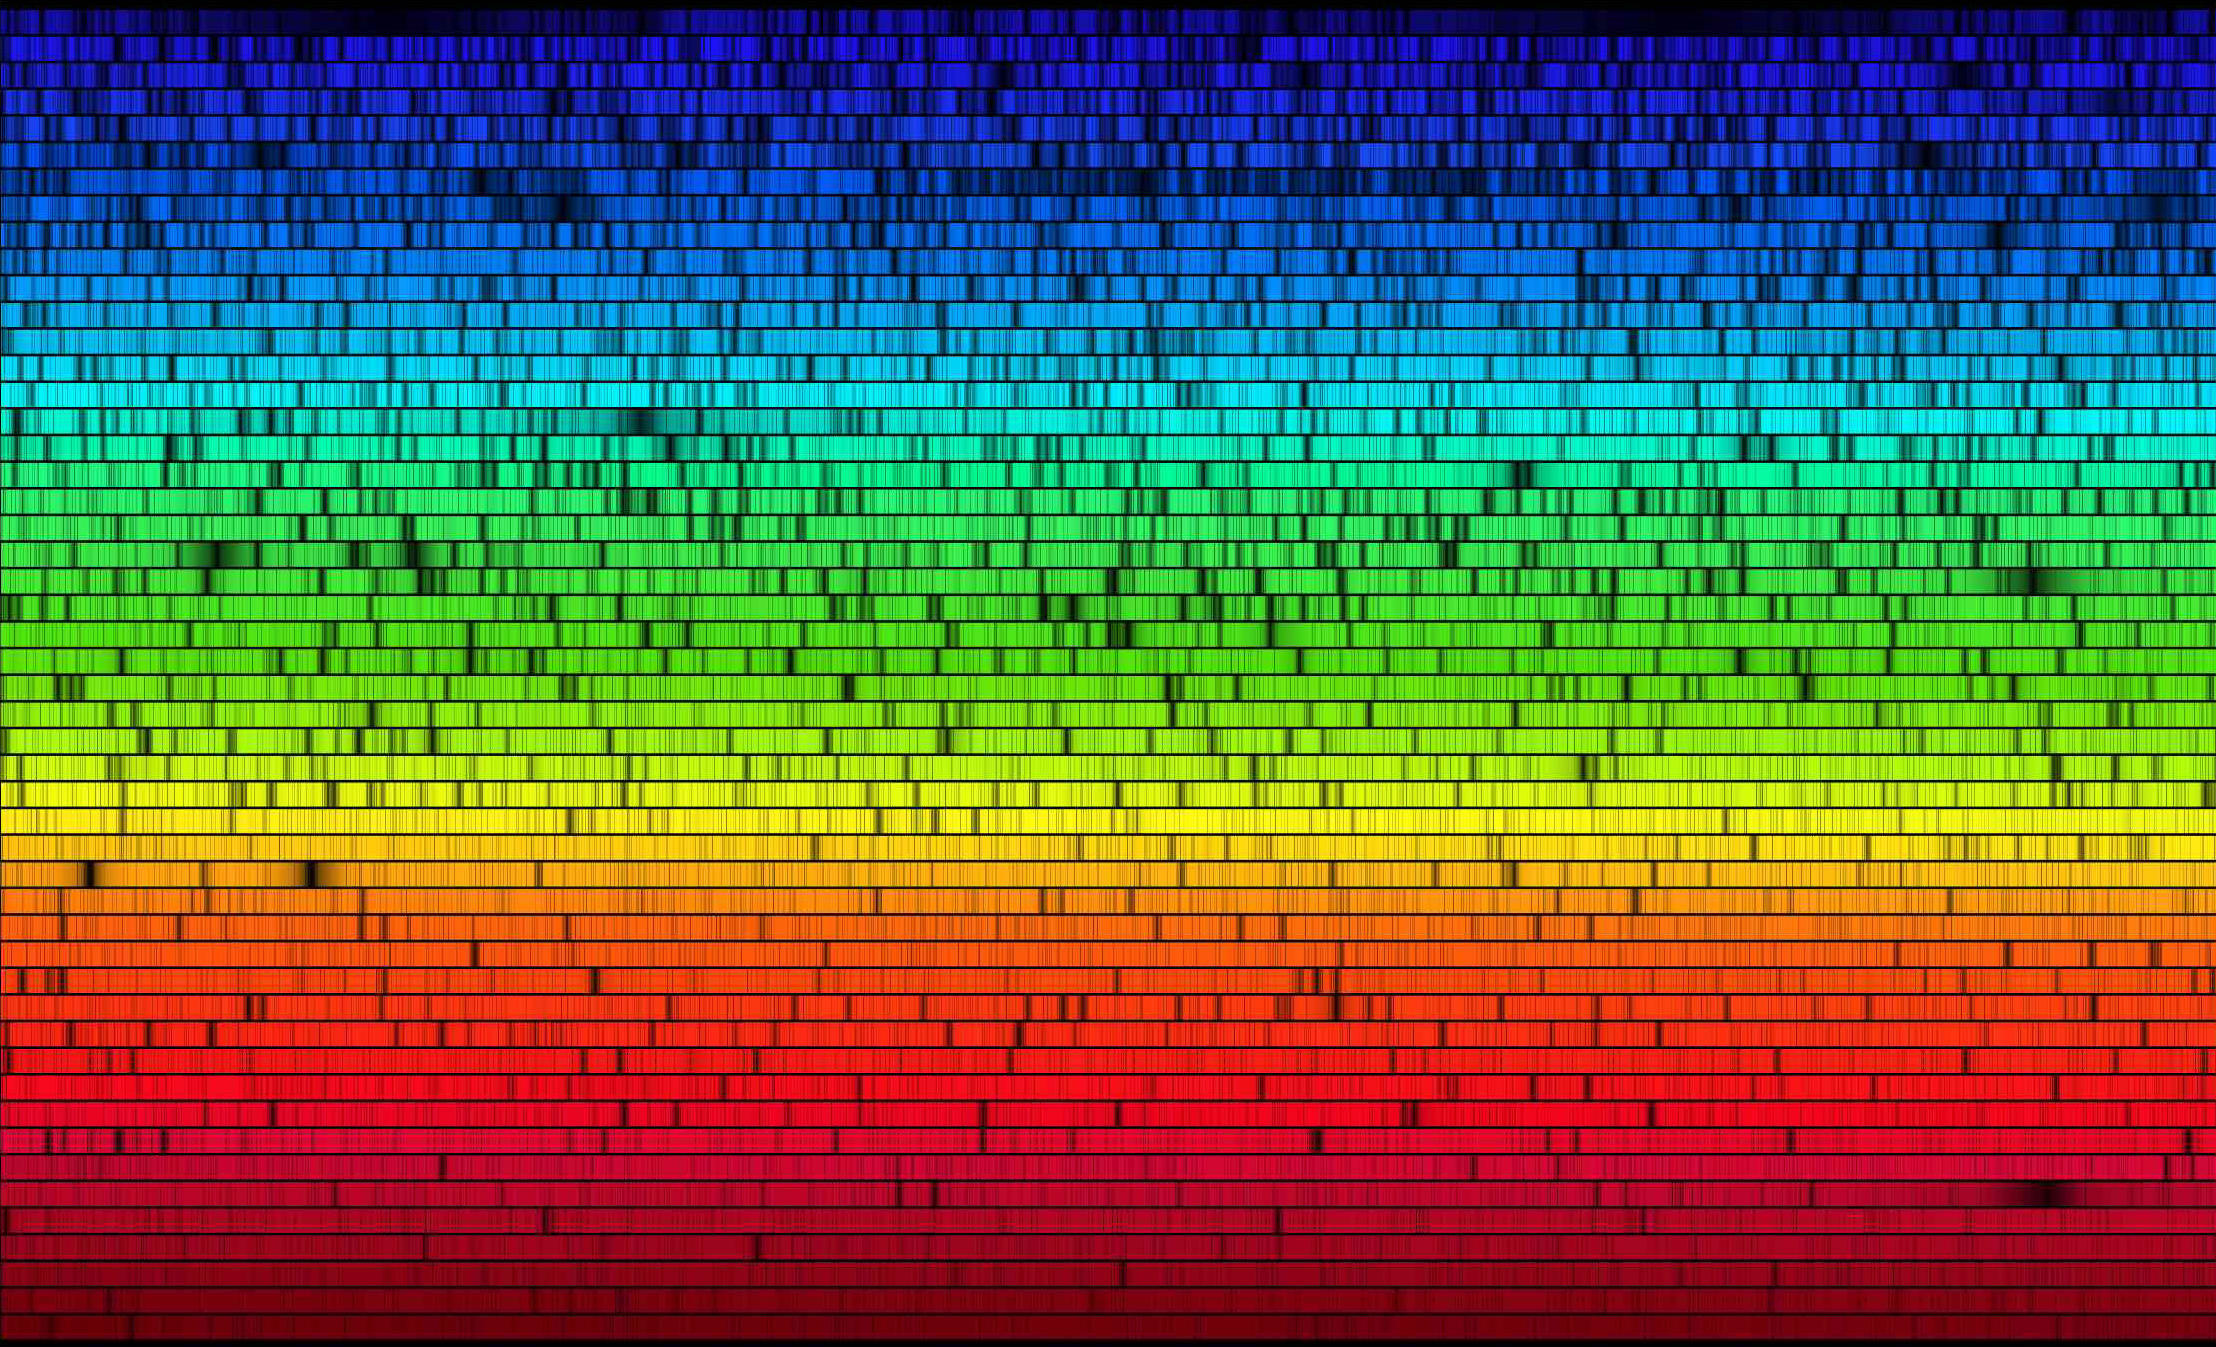
\includegraphics[width=130mm]{images/solar_spectra}
	
}


\frame[t]
{
%...................................................................................................
\note<1>[]{So we run simulations of the sun w/ and w/o lines and get the this result. But before we pay attention to the plot, let me explain...so we can see the lines really are the main contributor to the TSI variability}
%...................................................................................................
	\frametitle{Importance of lines for variability}
	\begin{itemize}
		\item TSI -- \alert{T}otal \alert{S}olar \alert{I}rradiance, i.e. integrated over wavelengths
		\item SSI -- \alert{S}pectral \alert{S}olar \alert{I}rradiance, depends on wavelength 
		\item $\triangle$ -- difference between the solar minima and maxima
		%\item The increase of the TSI at maximum of the activity cycle compared with minimum is directly attributed to the variability in spectral lines
	\end{itemize}
	\centering
	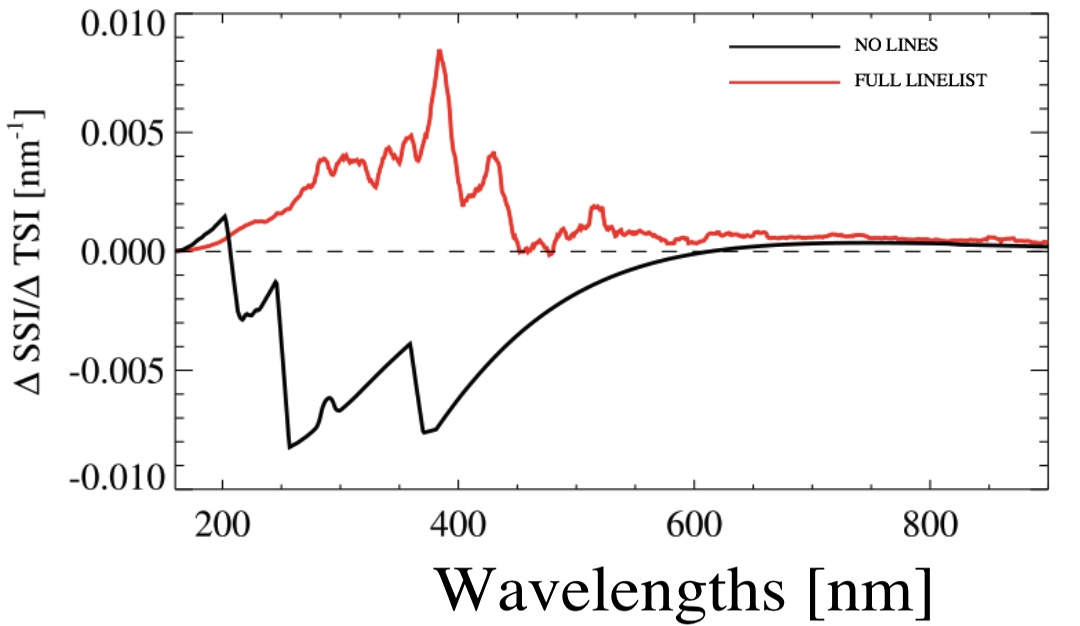
\includegraphics[width=90mm]{images/continuum}
}


\frame[t]
{
%...................................................................................................
\note<1>[]{}
%...................................................................................................
	\frametitle{Importance of lines for variability}
	\vspace{2.1em}
	\centering
	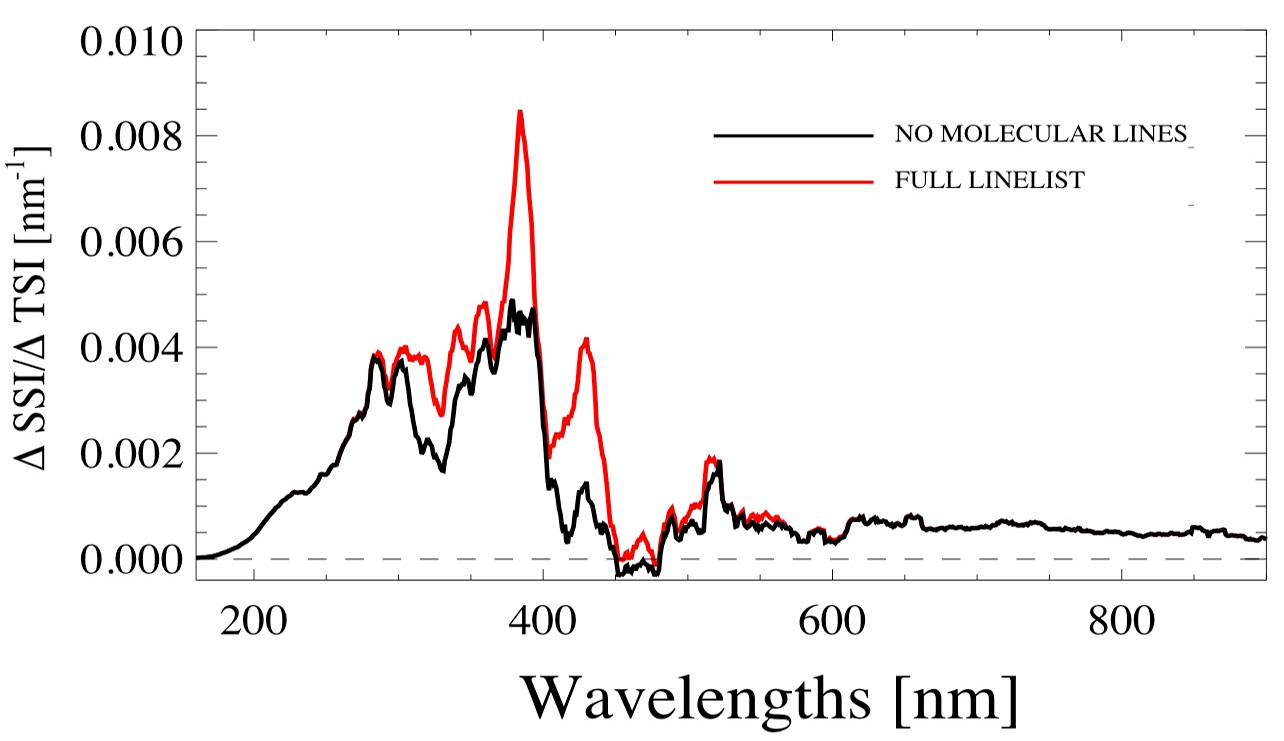
\includegraphics[width=.73\textwidth]{images/timescales_2}
}


\frame[t]
{
%...................................................................................................
\note<1>[]{...careful and appropriate treatment of spectral lines is necessary for TSI variability calculations.}
%...................................................................................................
	\frametitle{Importance of lines for variability}
	\begin{itemize}
		\item \alert{25\%} of the variability comes from molecular lines $\rightarrow$ accurate treatment of lines is crucial
	\end{itemize}
	\centering
	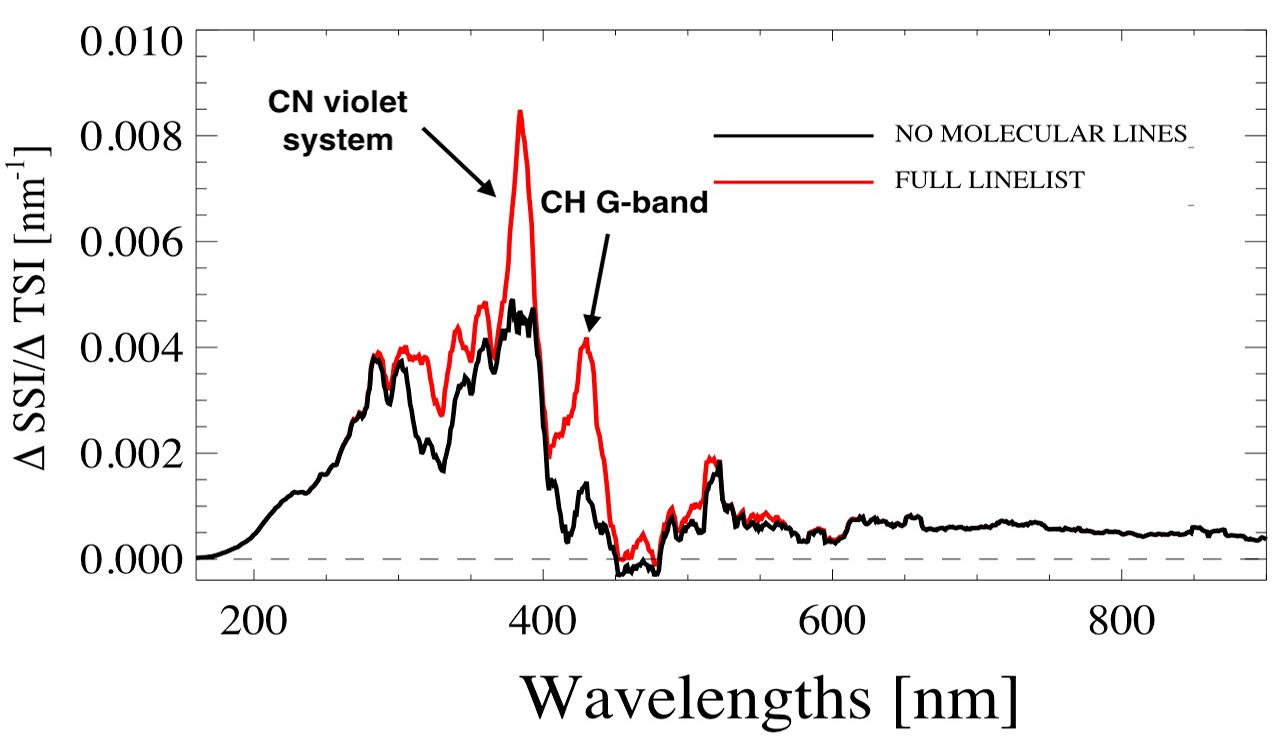
\includegraphics[width=.73\textwidth]{images/timescales_3}
}





%%...................................................................................................
%\note<1>[item]{The Str\"omgren filters B and Y, as well as the Kepler passband or the COROT filter, are broadly used for observations.
%
%Therefore, these filters are of particular interest when radiative transfer calculations are performed. Currently, this is computationally demanding due to a huge amount of atomic and molecular lines.
%
%In this talk, I will show that a SIGNIFICANT speed up can be achieved by using optimized opacity detribution functions, which we call OODF!
%
%Let’s start with the example of the Strömgren Y filter. As you can see the intensity is dominated by lines….}

\frame
{
%...................................................................................................
\note<1>[]{ODFs are useful for many applications (among them variability calculations) which require a low resolution flux/intensity. I am interested in calculating the  flux from some part of the spectra, which I will call the bin}
%...................................................................................................
	\frametitle{Generating ODFs}
	\begin{itemize}
    \item Start with high resolution opacity	
	\end{itemize}

	\centering
	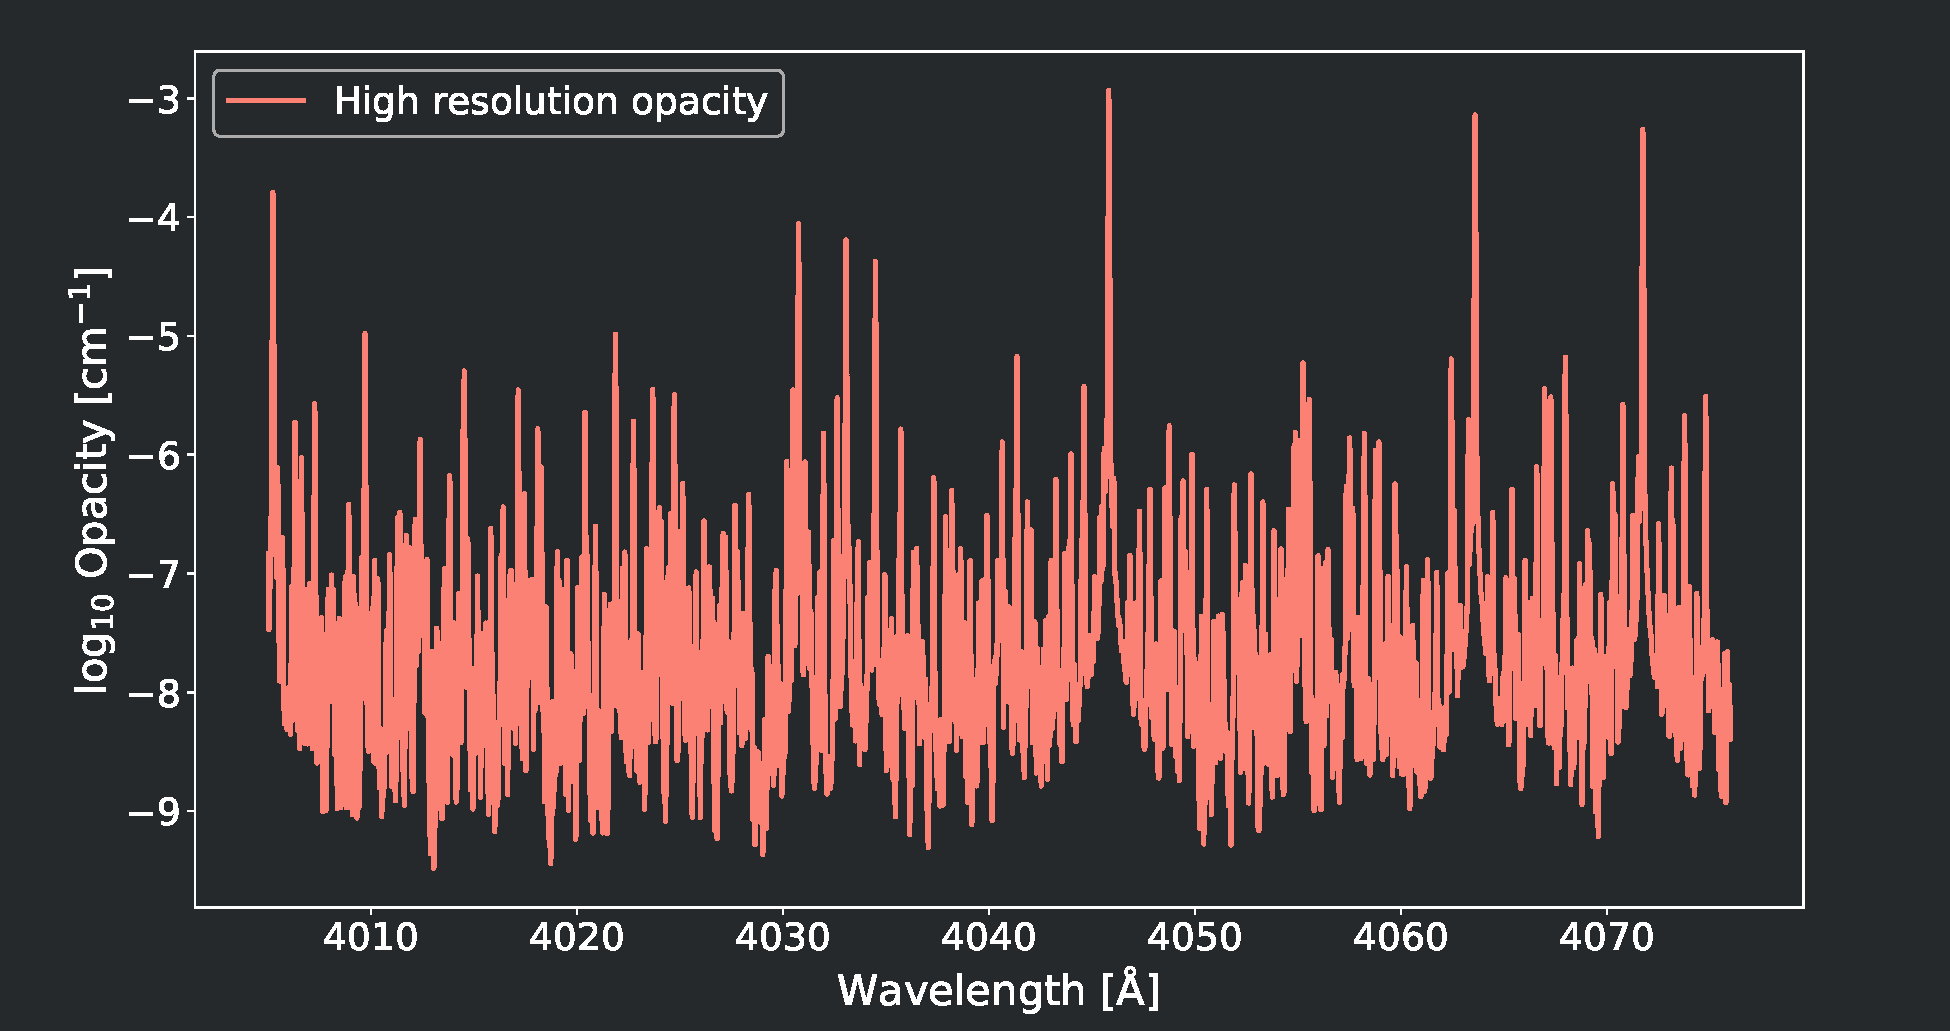
\includegraphics[width=130mm]{images/odf_generation_process_0}
}

\frame
{
%...................................................................................................
\note<1>[]{}
%...................................................................................................
	\frametitle{Generating ODFs}
	\begin{itemize}
    \item Sort wavelength points by corresponding values of opacity; monotonically increasing opacity
    \item Integral is preserved by sorting
	\end{itemize}		
	\centering
	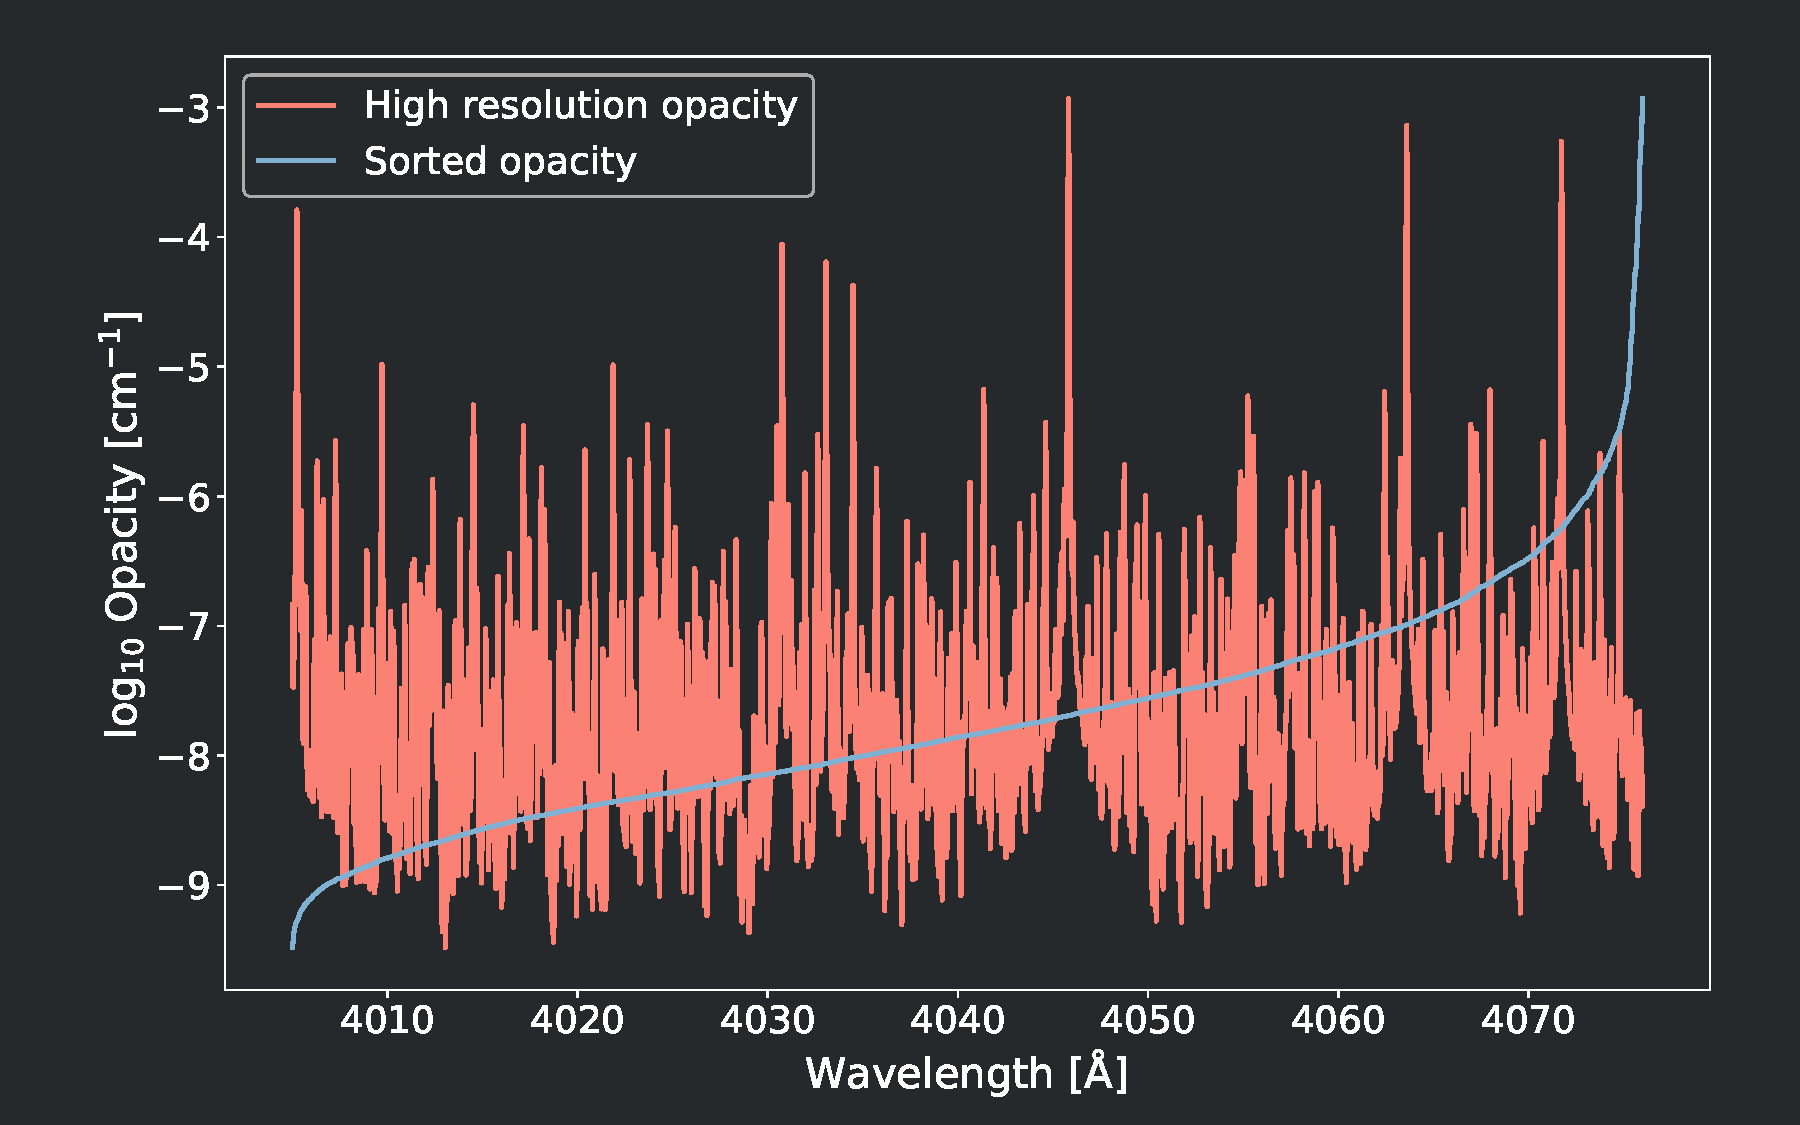
\includegraphics[width=123mm]{images/odf_generation_process_1}
}

\frame
{
%...................................................................................................
\note<1>[item]{Take notes here.}
%...................................................................................................
	\frametitle{Generating ODFs}
	\begin{itemize}
		\item All wavelength information within the bin is lost
\end{itemize}		

		\centering
	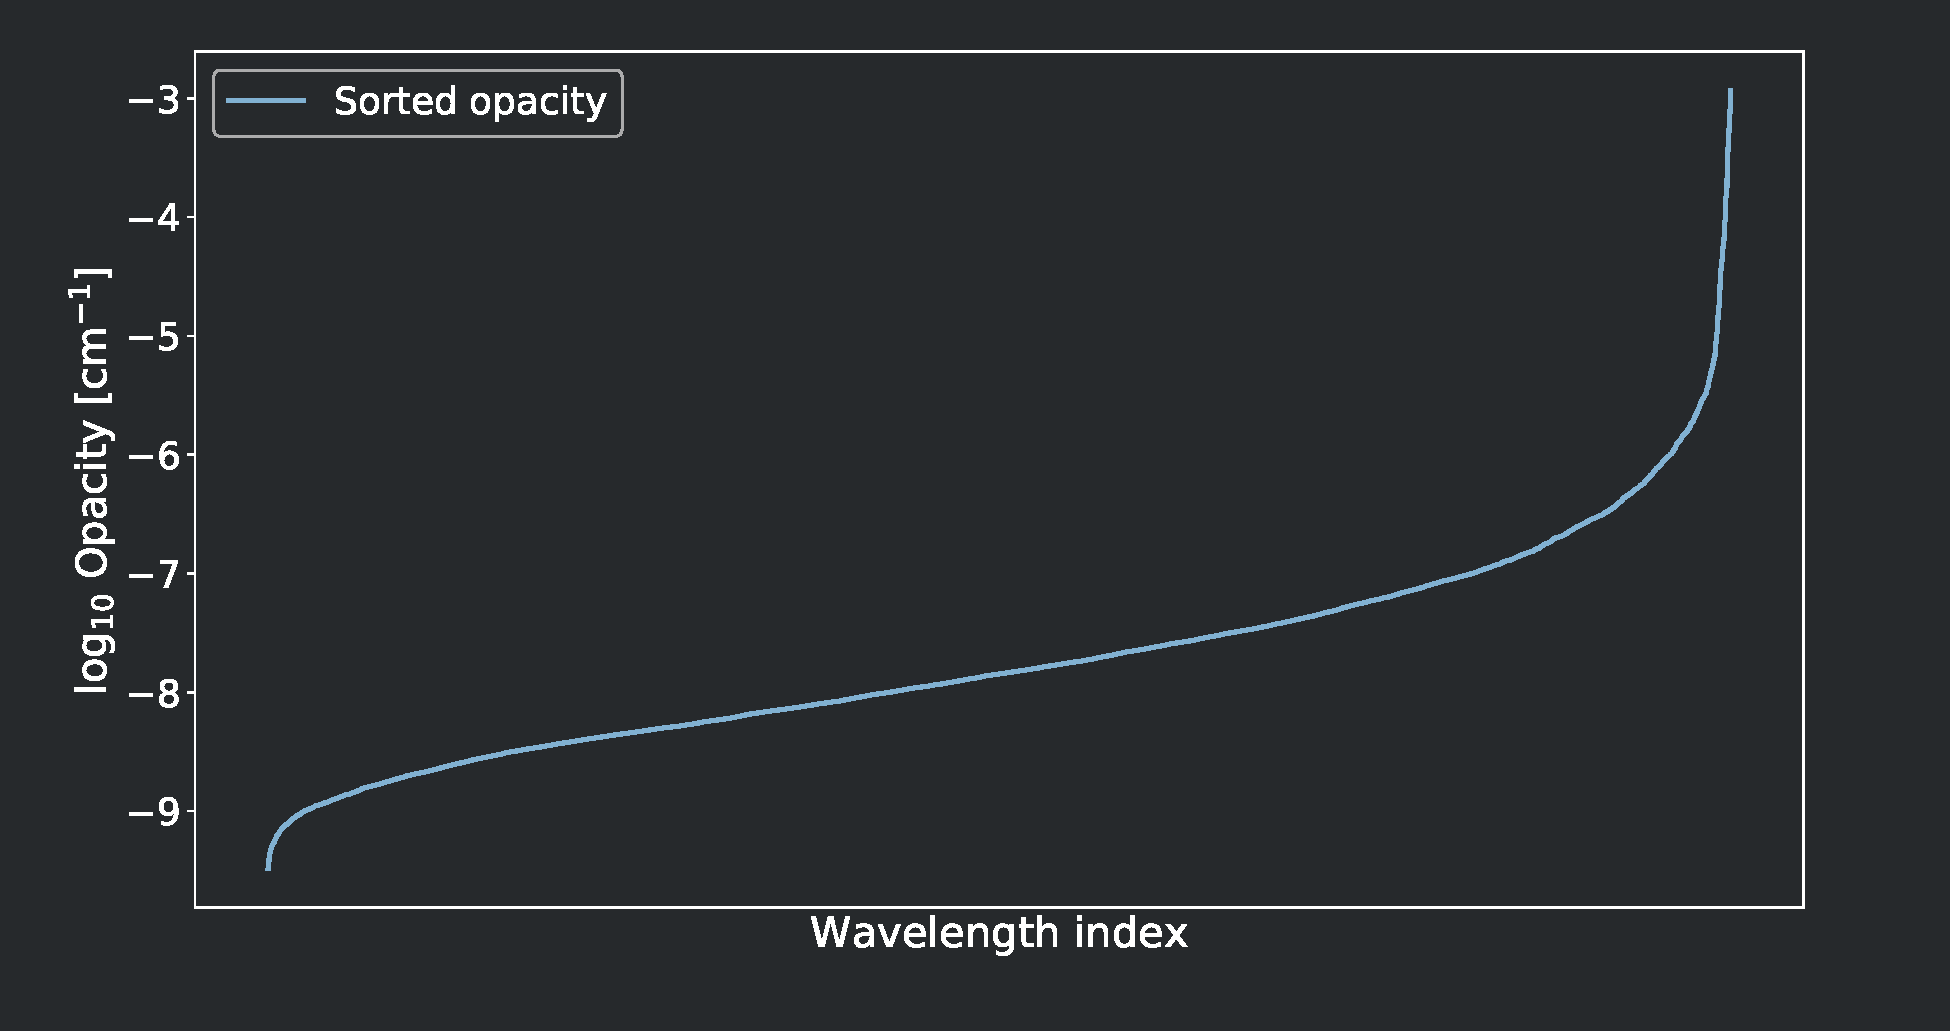
\includegraphics[width=130mm]{images/odf_generation_process_2}
}

\frame
{
%...................................................................................................
\note<1>[]{}
%...................................................................................................
	\frametitle{Generating ODFs - Example with 10 uniform sub bins}
	\begin{itemize}
		\item Approximate the sorted opacity with a step-wise function
	\end{itemize}
	\centering
	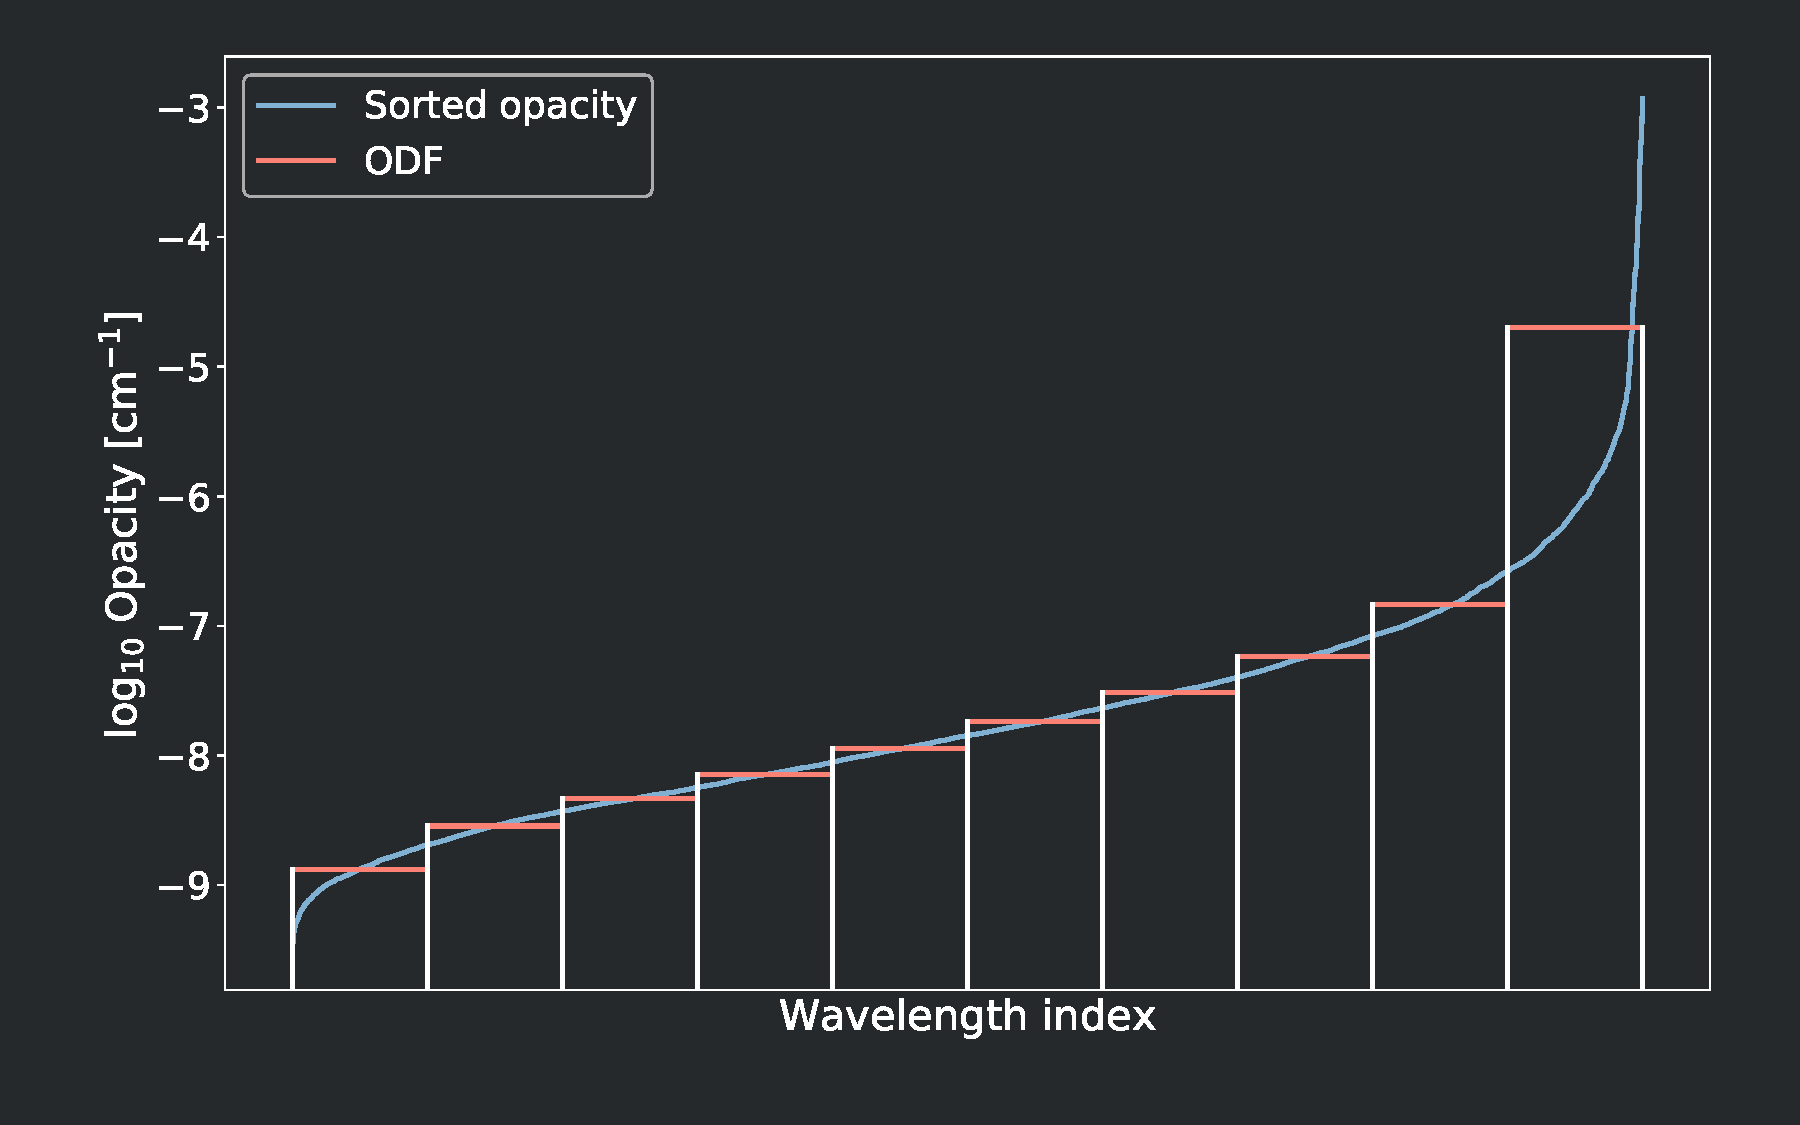
\includegraphics[width=130mm]{images/odf_generation_process_3}
}
\frame
{
%...................................................................................................
\note<1>[]{}
%...................................................................................................
	\frametitle{ODF generation process}
	\begin{itemize}
	\item Mean is skewed by extreme values
	\end{itemize}
	\centering
	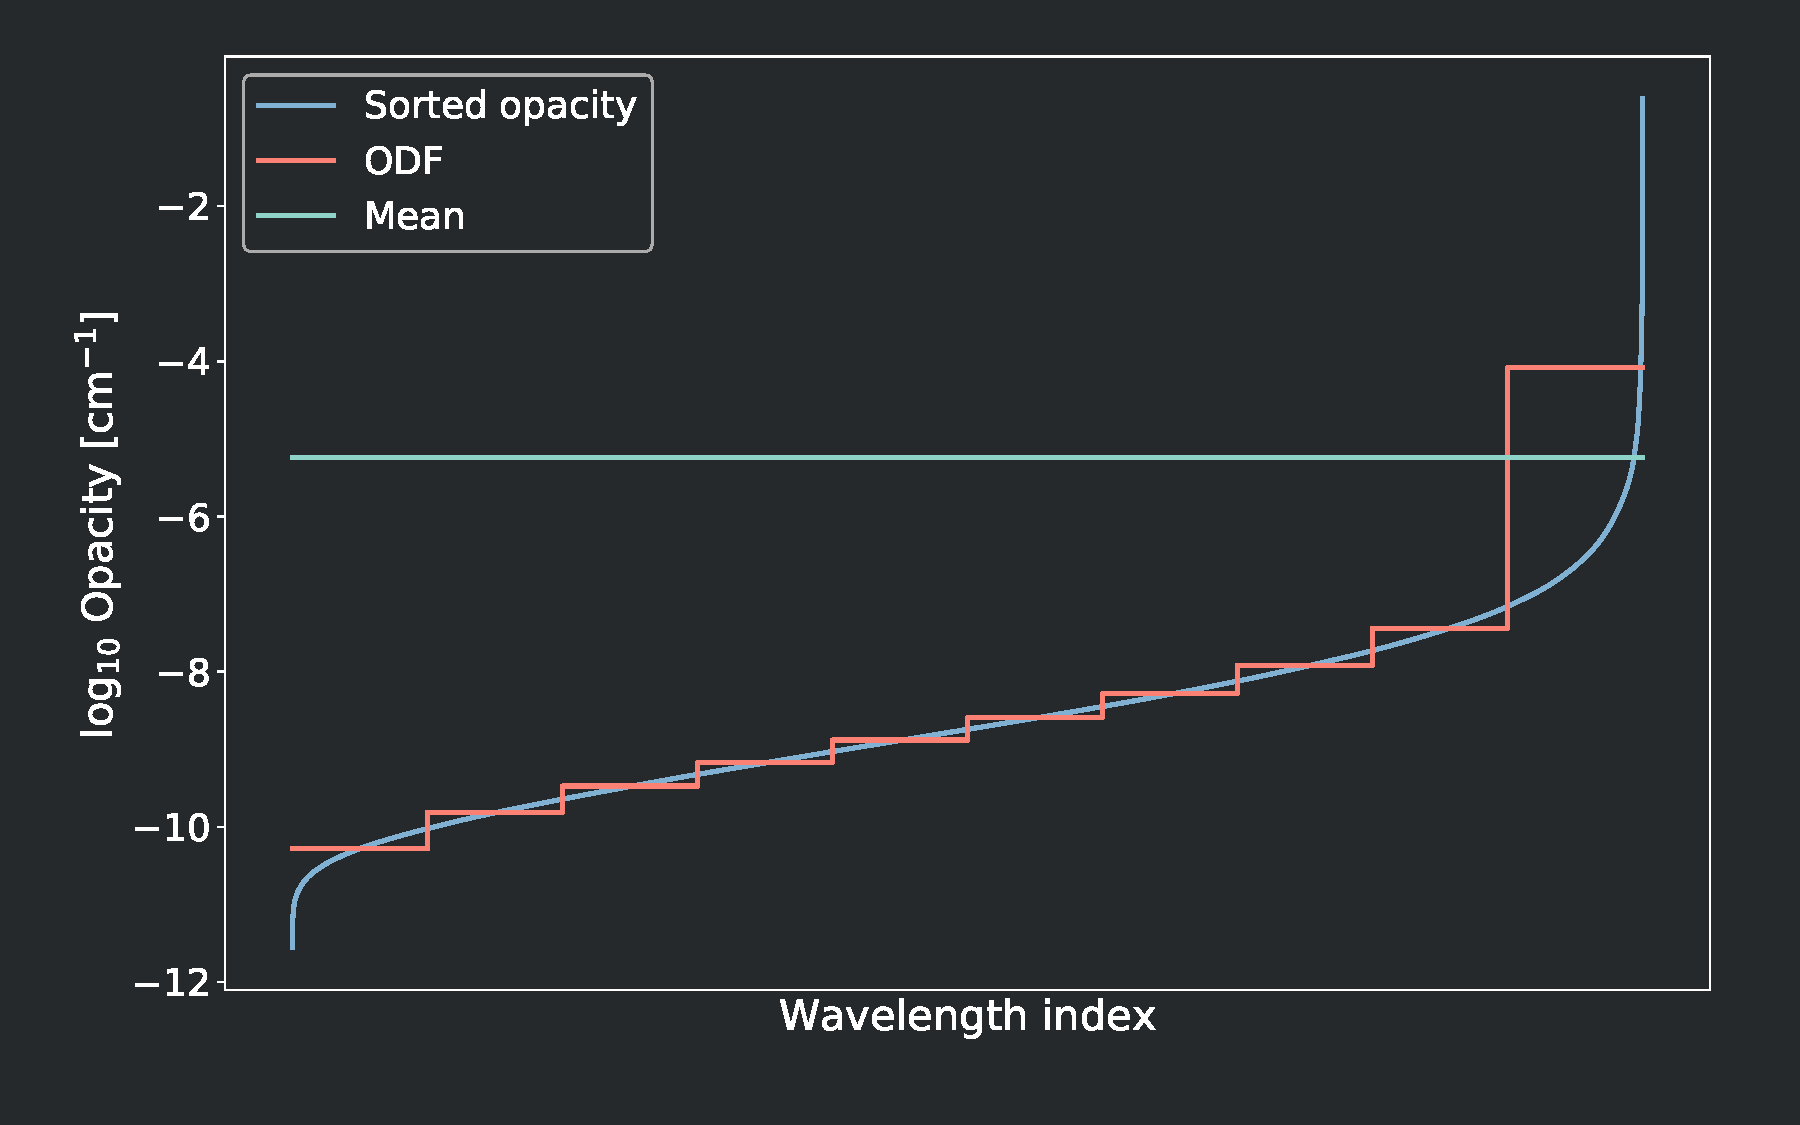
\includegraphics[width=130mm]{images/odf_generation_process_4}
}

\frame
{
%...................................................................................................
\note<1>[]{}
%...................................................................................................
	\frametitle{ODF performance analysis}
	\begin{itemize}
	    \item Synthesize spectra with \textbf{NESSY} radiative transfer code using ODFs from 1000-9000\si{\angstrom} in 10\si{\angstrom} bins
	    \item Compare the fluxes from the ODF spectrum with the high resolution spectrum in the bins
	\end{itemize}
	\centering
	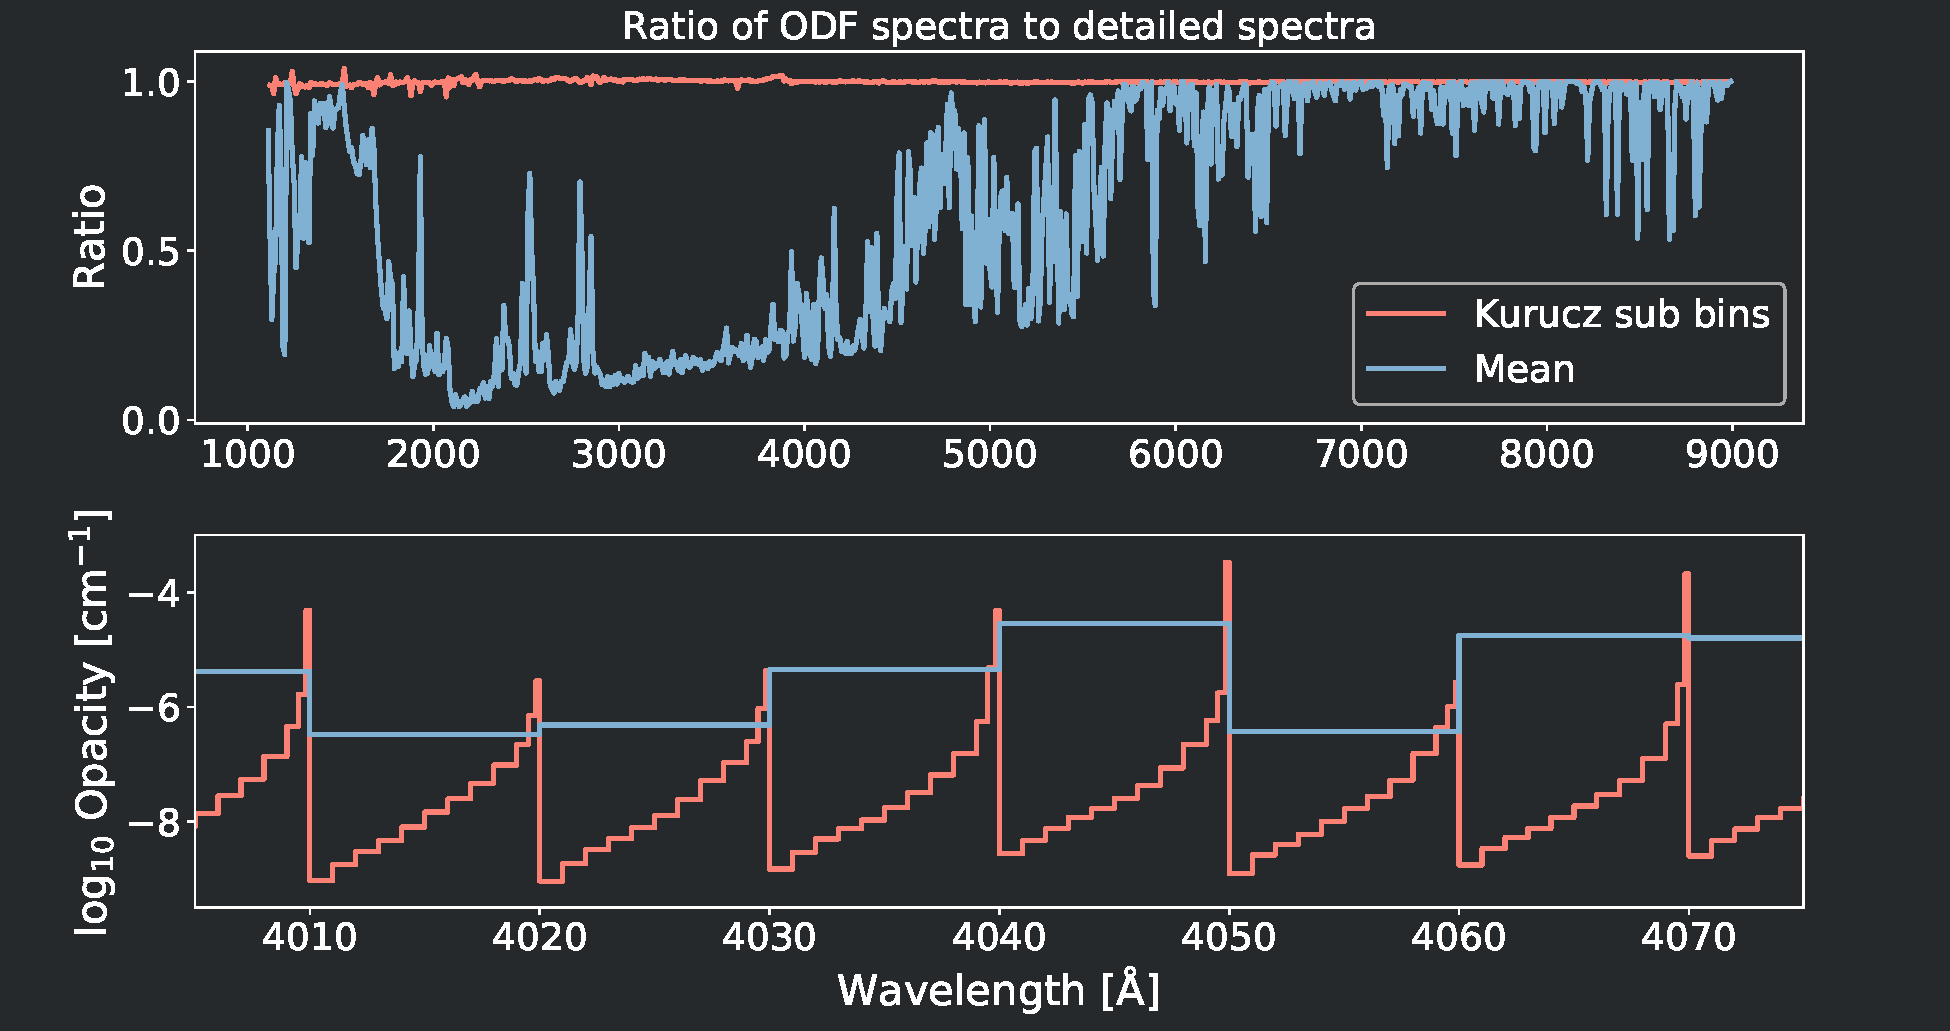
\includegraphics[width=120mm]{images/odf_vs_non_odf}
}


\frame[t]
{
%...................................................................................................
\note<1>[]{}
%...................................................................................................
	\frametitle{Possible solutions}
	\large{Number of calculations $\mathrm{n_{cal} = n_{bins} \times n_{sub bins}}$}
	\vspace{4em}
	
	\centering
	
\begin{tikzpicture}[sibling distance=25em,
  every node/.style = {shape=rectangle, rounded corners,
    draw, align=center, color=white!20}]]
  \node {\Large{decrease $\mathrm{n_{cal}}$ by}}
    child { node {decrease the number\\ of sub bins per bin} }
    child { node {increase bin size \\
    				  $\rightarrow$ decrease $n_{bins}$} };
\end{tikzpicture}

%	\includegraphics[width=115mm]{images/}
}


\frame
{
%...................................................................................................
\note<1>[item]{}
%...................................................................................................
	\frametitle{Analysis of different ODFs}
	\begin{itemize}
	\item Uniform ODFs
	\end{itemize}
	
	\centering
	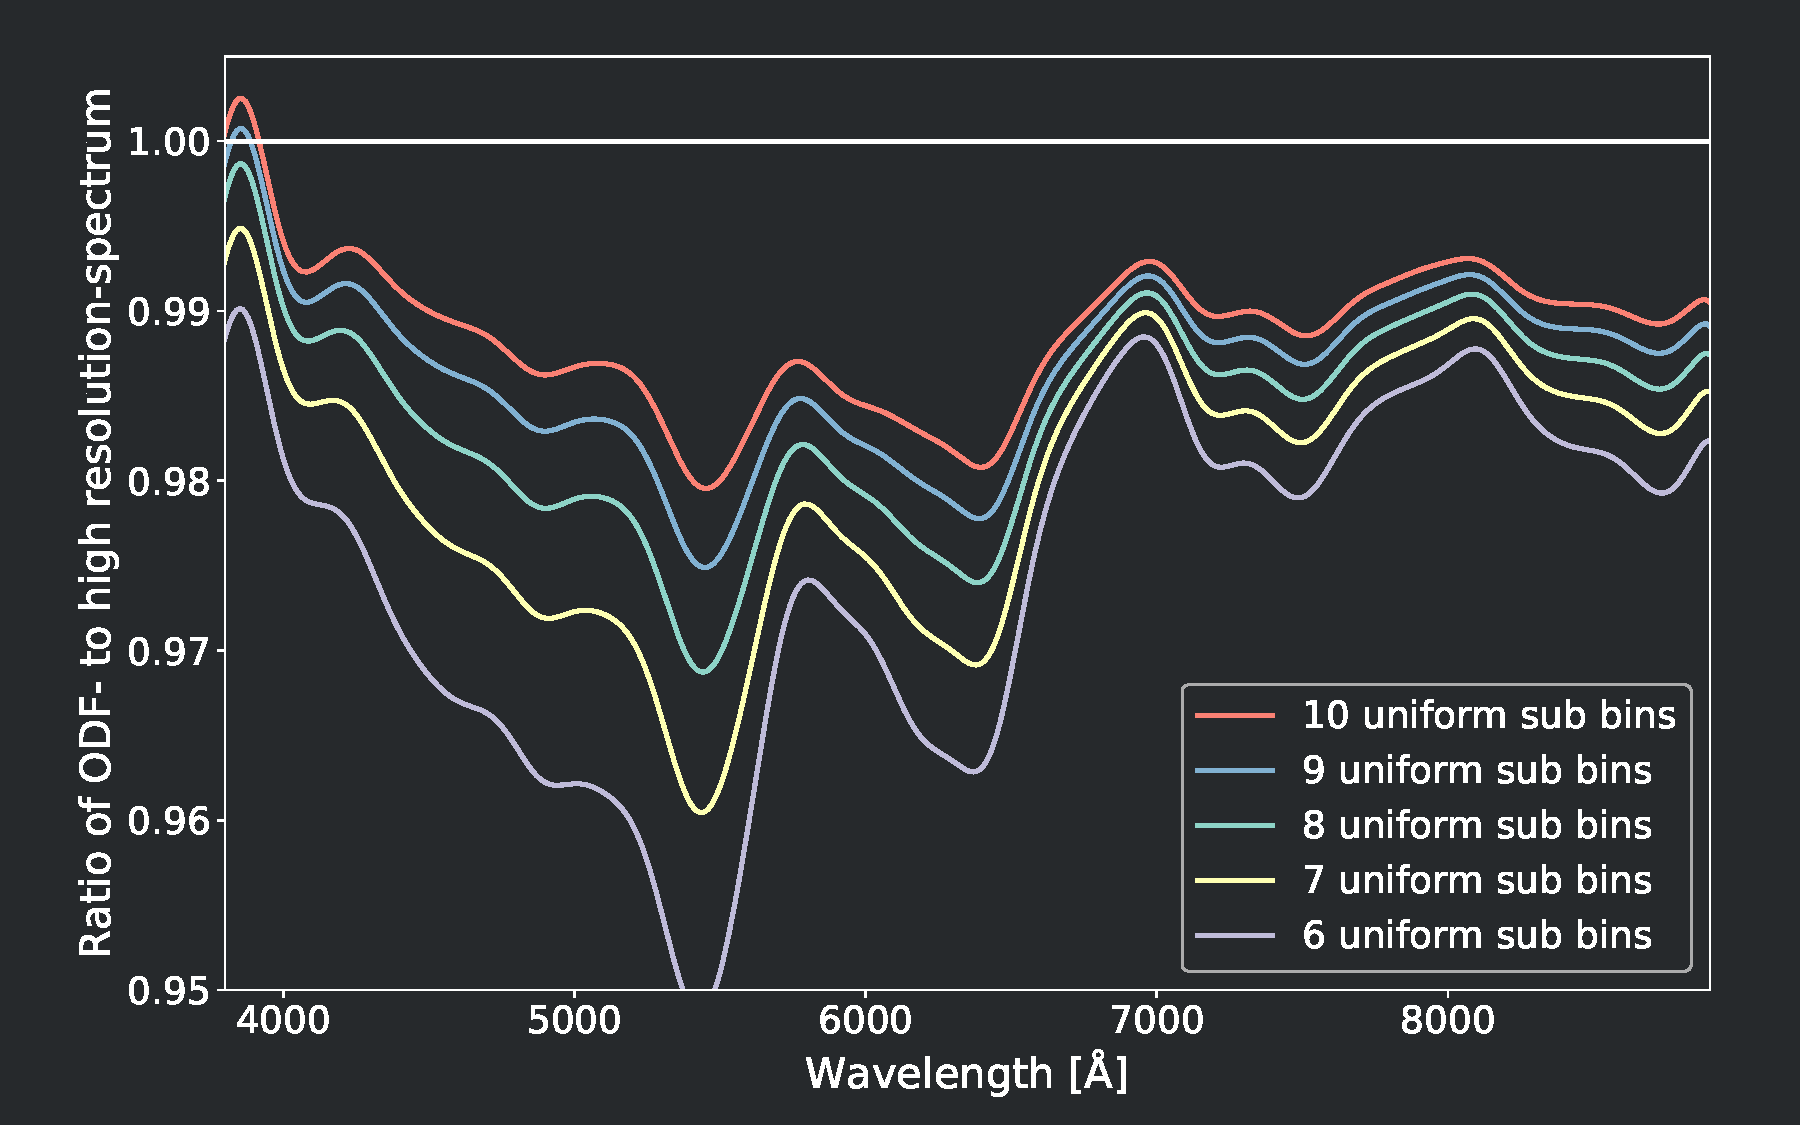
\includegraphics[width=130mm]{images/6_10_vs_best_4_0}
}
\frame
{
%...................................................................................................
\note<1>[]{}
%...................................................................................................
	\frametitle{Analysis of different ODFs}
	\begin{itemize}
		\item Nonuniform ODFs
		\item The last sub bin is crucial after 5000\si{\angstrom}
    \end{itemize}	  
	\centering
	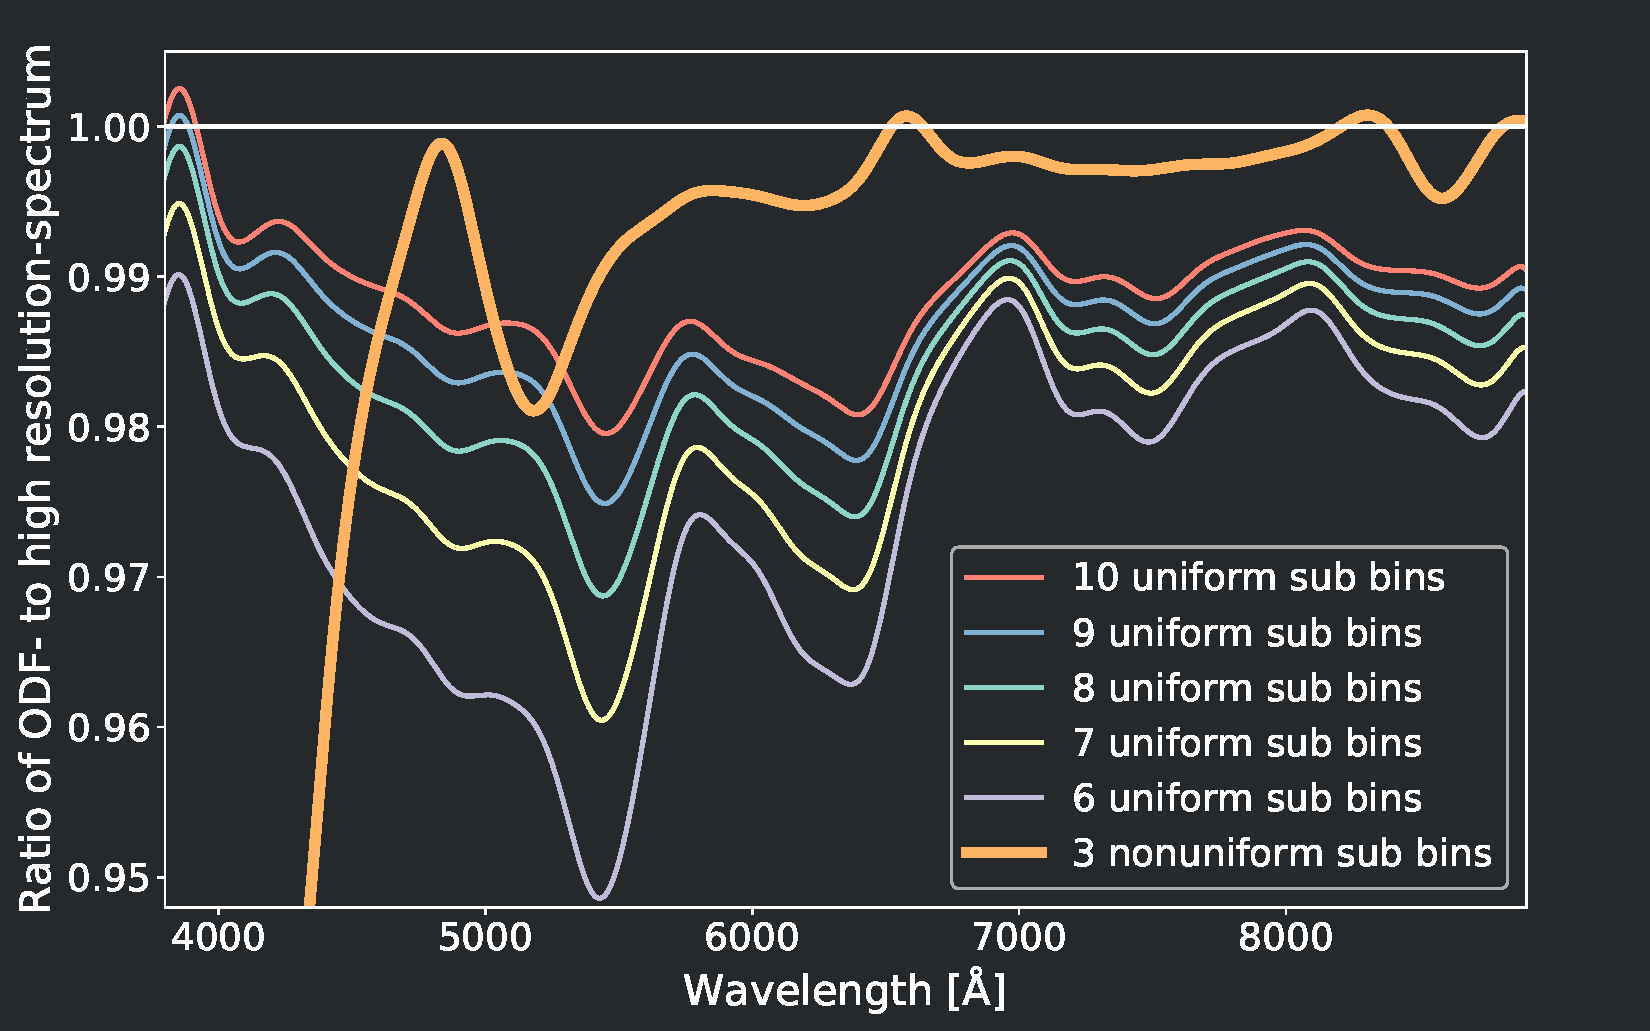
\includegraphics[width=120mm]{images/6_10_vs_best_4_1}
}
\frame
{
%...................................................................................................
\note<1>[]{}
%...................................................................................................
	\centering	
	\frametitle{Best sub bin combinations using 4 sub bins}
	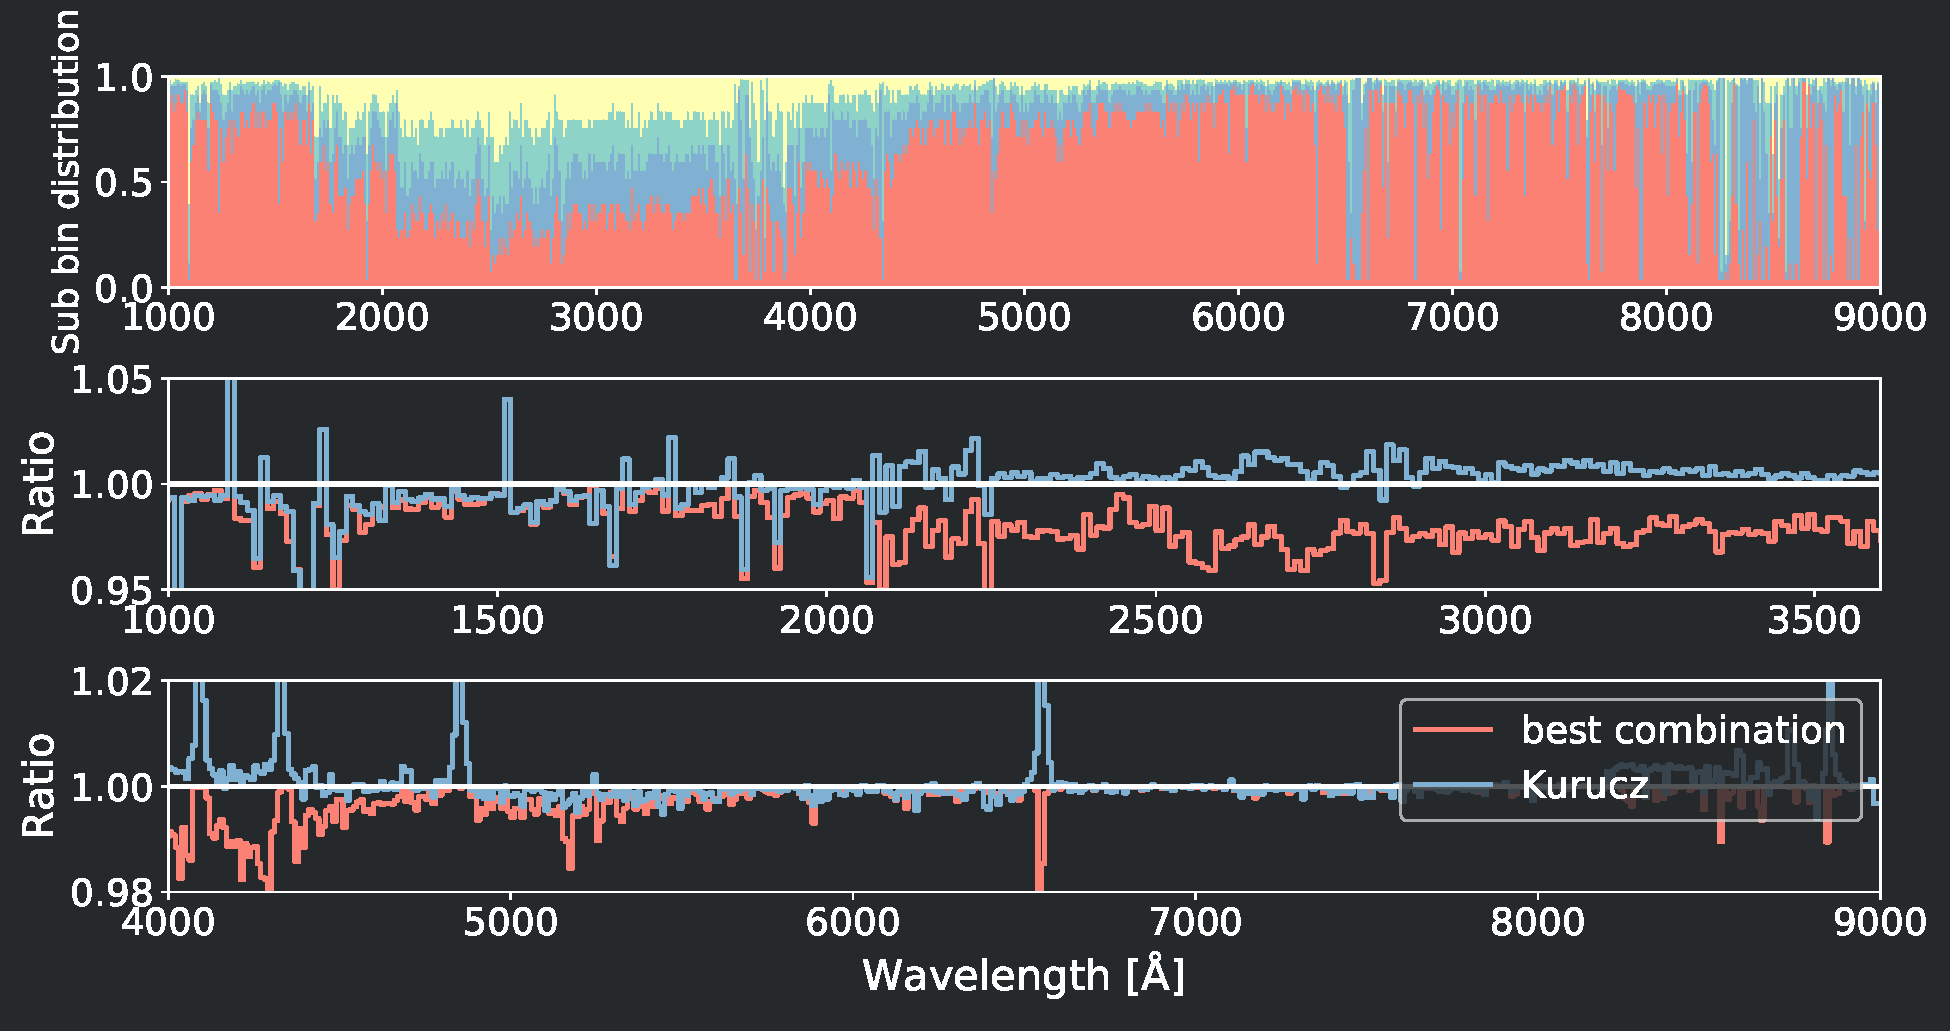
\includegraphics[width=140mm]{images/best_combination_finder_0}
}

%\frame
%{
%%...................................................................................................
%\note<1>[]{}
%%...................................................................................................
%	\centering		
%	\frametitle{Best sub bin combinations using 10 sub bins}
%	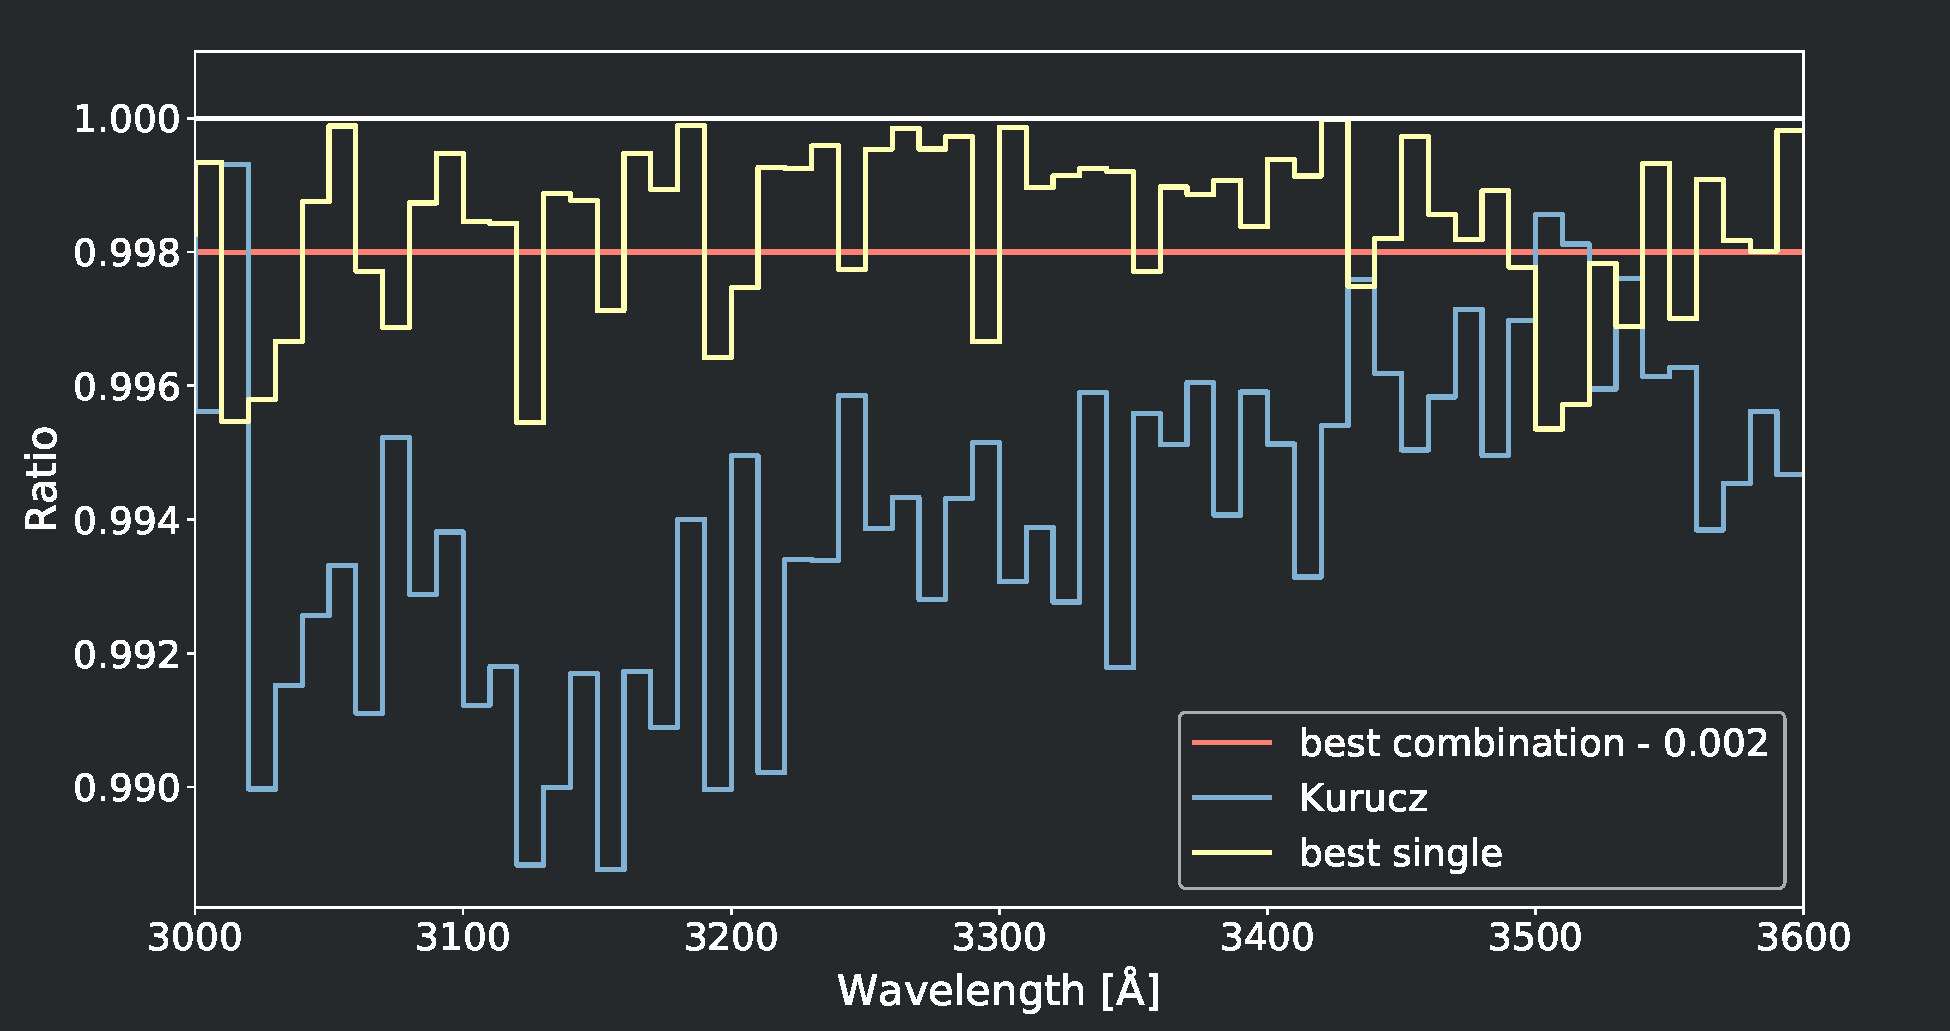
\includegraphics[width=130mm]{images/best_combination_finder_10_1}
%}


\frame
{
%...................................................................................................
\note<1>[]{}
%...................................................................................................
	\frametitle{Str\"omgren \textit{b}}
	\centering
	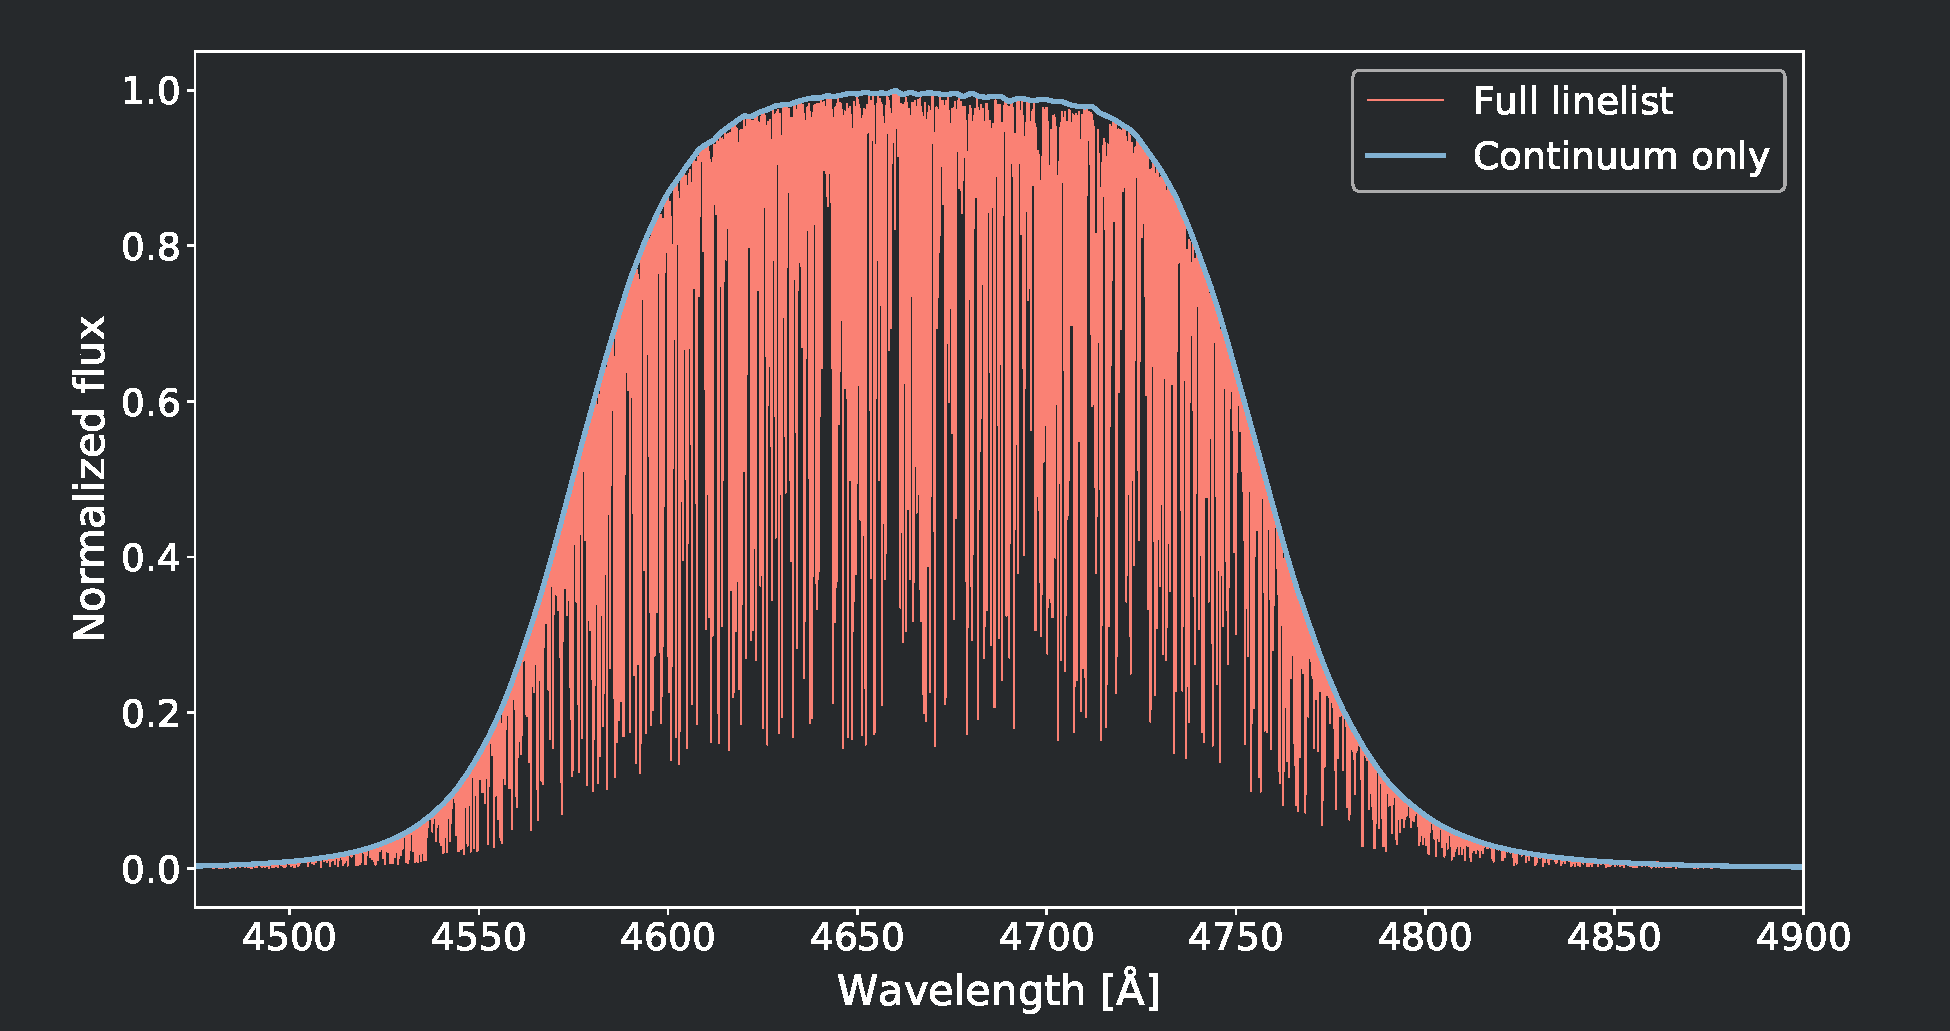
\includegraphics[width=140mm]{images/b_filter}
}


\frame
{
%...................................................................................................
\note<1>[]{}
%...................................................................................................
	\frametitle{OODF treatment of filters}
	\begin{itemize}
		\item ODF approach can be generalized to take into account any shape of transmission function
		\item Achieved by transforming the wavelength grid according to the transmission function
	\end{itemize}
	\centering
	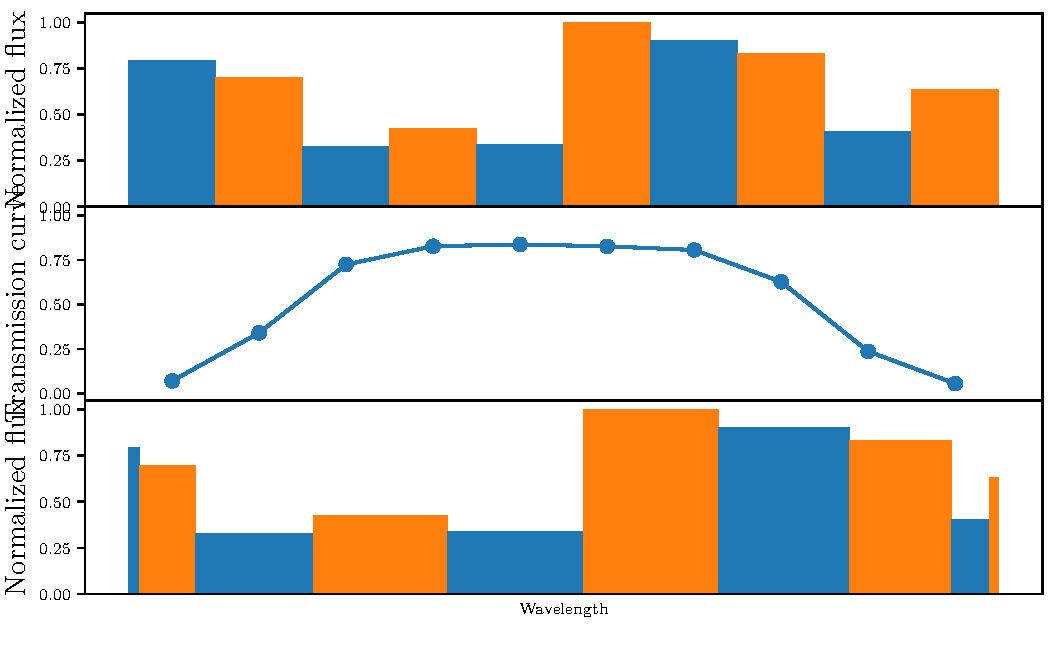
\includegraphics[width=130mm]{images/odf_filters}
}


\frame
{
%...................................................................................................
\note<1>[]{}
%...................................................................................................
	\frametitle{Speedups in the case of Str\"omgren \textit{b}}
	\begin{itemize}
		\item Interval length (transmission curve > 1\%): $\sim$400\si{\angstrom} \\[20pt]
	\end{itemize}
	
	\centering
%	High resolution calculation 80 points per \si{\angstrom} $\sim$ 80 000 \\
%	ODF calculations 12 points per 10\si{\angstrom} $\sim$ 1200 \\
%	OODF calculations 3 points per 1000\si{\angstrom} $\sim$ 3 \\

\begin{tikzpicture}[sibling distance=25em,
  every node/.style = {shape=rectangle, rounded corners,
    draw, align=center, color=white!20}]]
  \node {\large{High resolution: 80 points per \si{\angstrom} $\sim$ 32 000 points}\\}
    child { node {ODF: 12 points per 10\si{\angstrom} $\sim$ 480 points \\
    \alert{\large{speedup 67 times}}} }
    child { node {OODF: 4 points for the whole bin \\
    \alert{\large{speedup $\sim$8 000 times}}} };
\end{tikzpicture}

}



\frame
{
%...................................................................................................
\note<1>[]{}
%...................................................................................................
	\frametitle{MSc project - Introduction}
    \large{Title: \textbf{Fast Approximate non-LTE Treatment of the Chromosphere}}
	\begin{itemize}
	\large{
		\item The aim of the magnetohydrodynamic group at my institute is  simulating the Sun from the upper part of the convection zone and up 
		\vspace{1em}
		%(convection zone, photosphere zone, chromosphere and corona) \\[10pt] 
		\\
			\centering 
	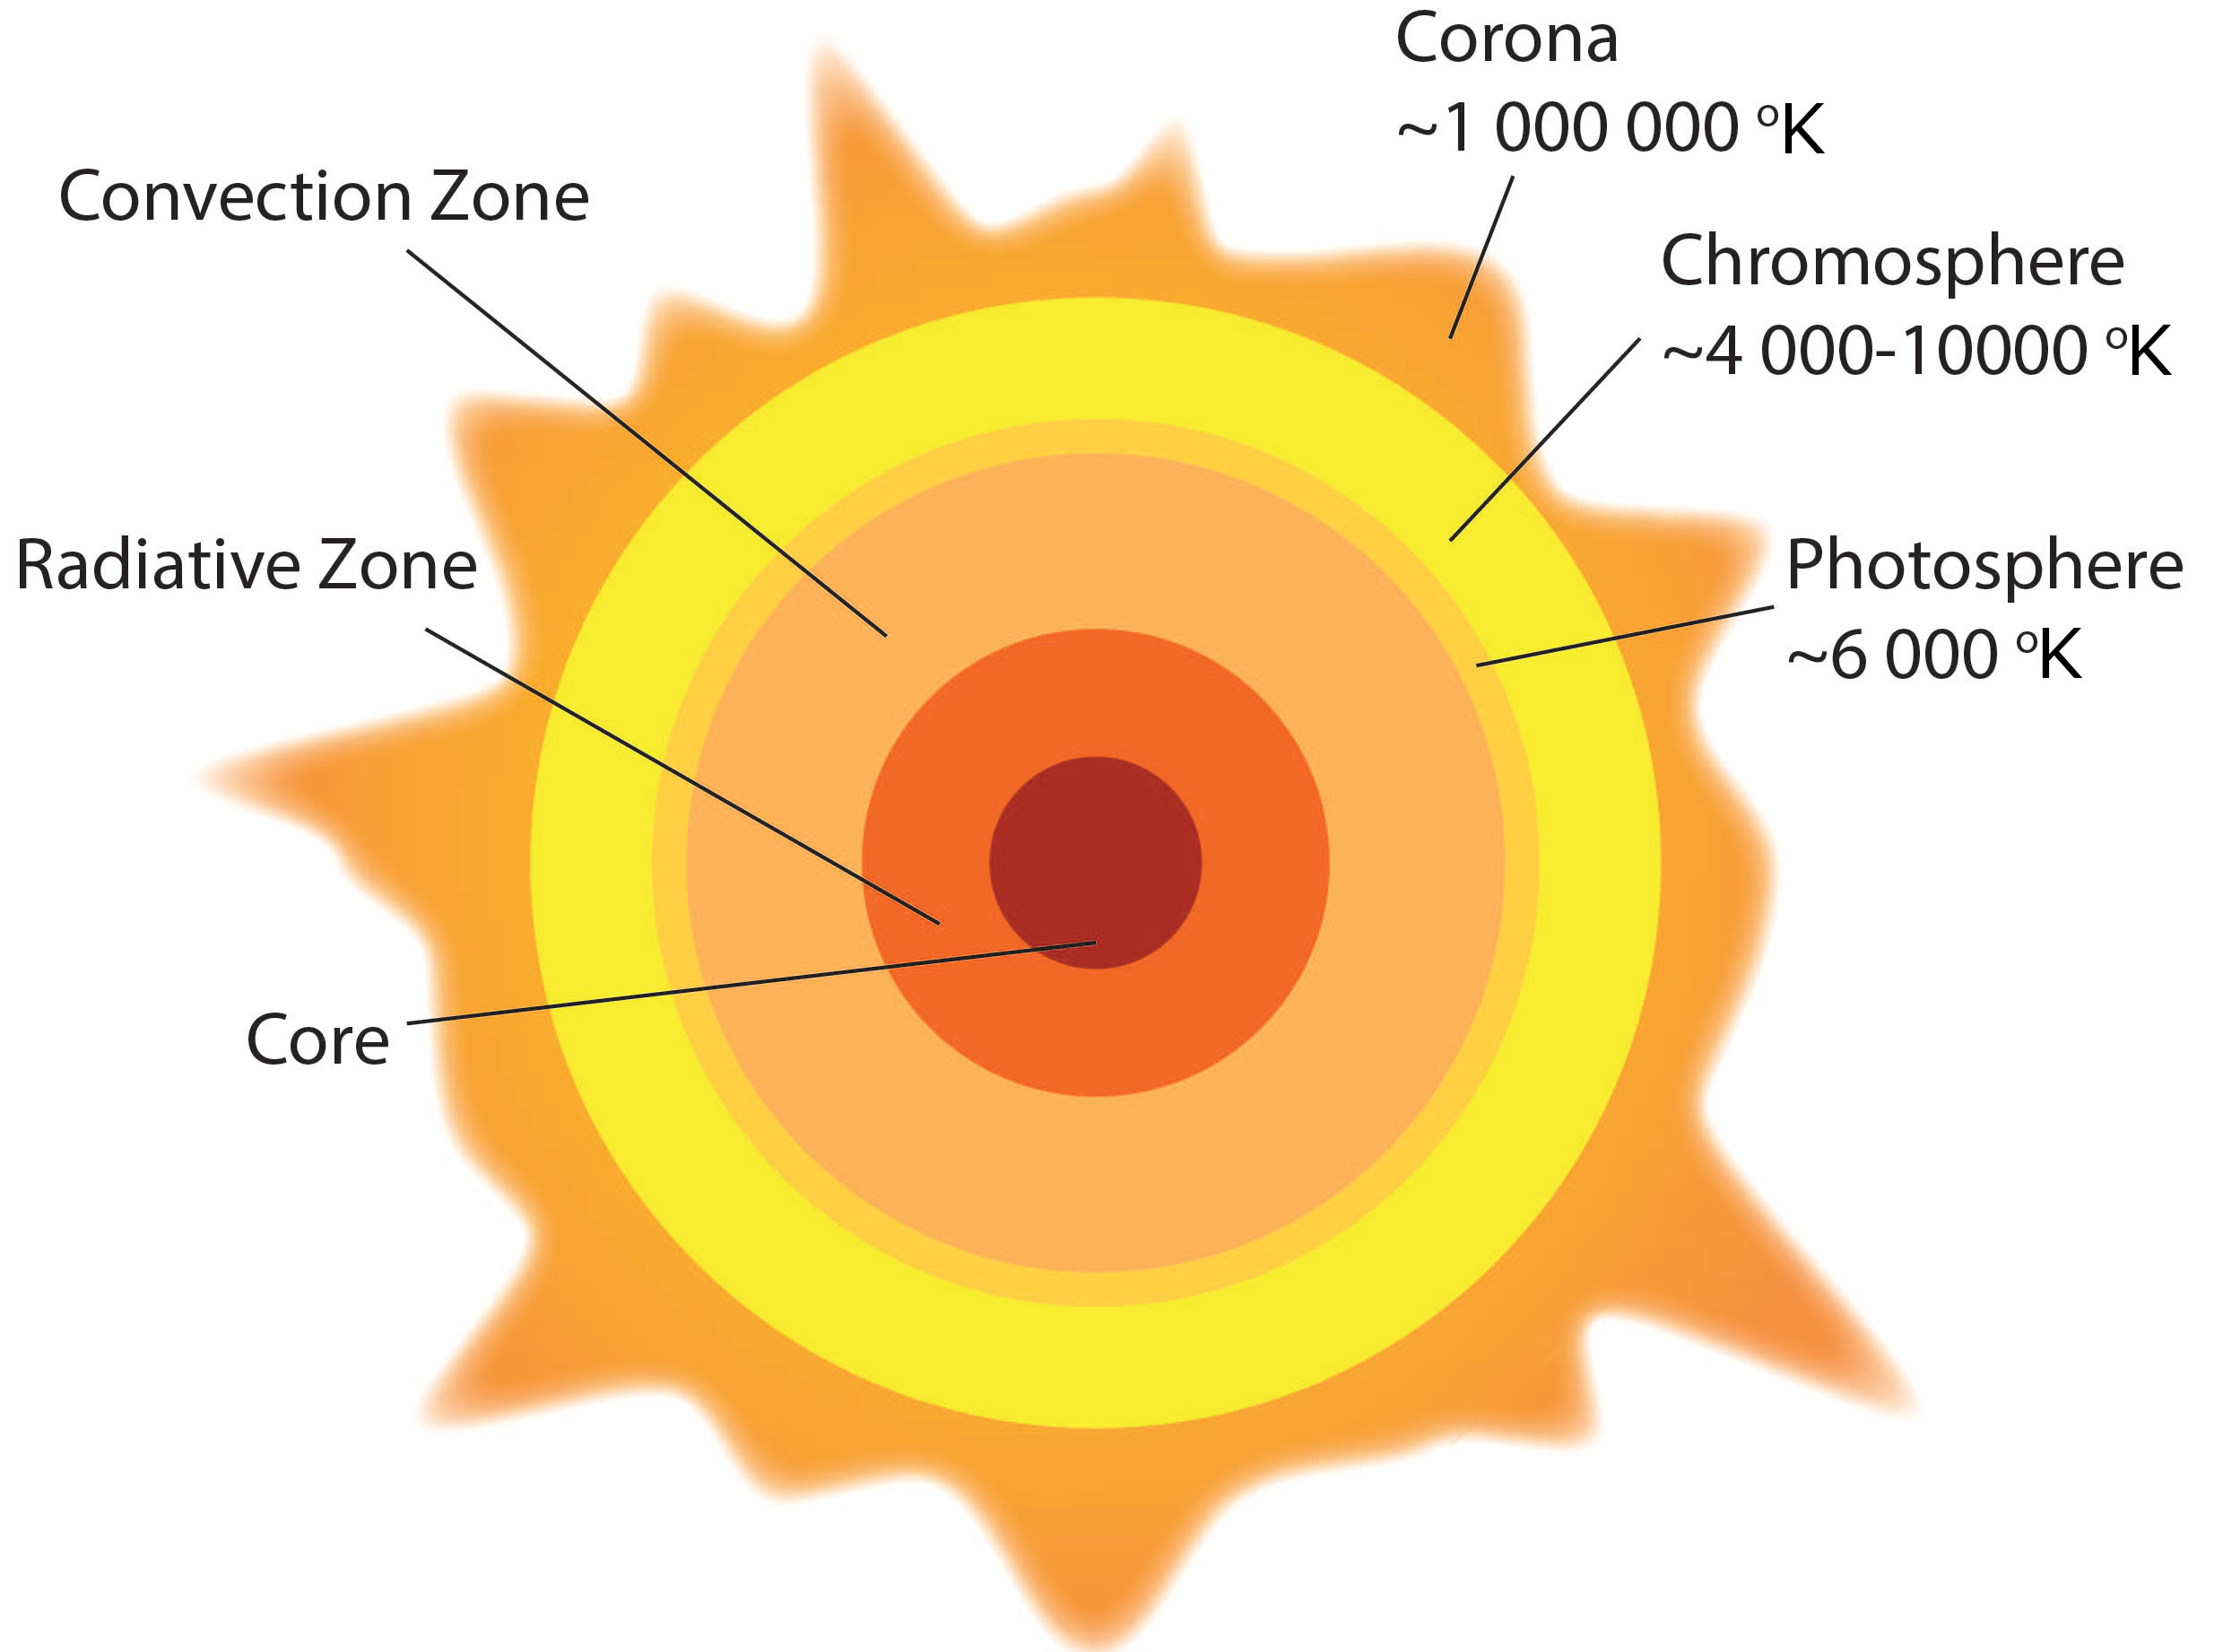
\includegraphics[width=60mm]{images/sun_structure}
	\url{http://www.phy.cuhk.edu.hk/elearning/Solar_eclipse/Solar_structure.html}

%		\item Corona is very hot, over 10$^6$K. Where does the heat come from? Coronal heating is an unsolved problem. \\[10pt] \pause
%		\item Chromosphere is dominated by non-LTE effects, a lot of energy loss due to ionization of H and He. \\[10pt] \pause
%		\item Full non-LTE treatment is time prohibitive, computational cost much larger than the MHD time step.

		%\item To properly treat this environment we must incorporate realistic radiative effects into large magnetohydrodynamic simulations. Cooling rates are currently approximated from large pre-calculated tables. The goal of my project is to calculate cooling rates using realistic radiative effects. I am implementing a new radiation solver into an existing C/C++ code. Starting with a single-core implementation for the 1D case, my goal is to implement MPI to address the full 3D problem. I will ultimately adapt the solver for a large scale MHD simulations on multi-GPU using openACC.

	}
	\end{itemize}
%	\centering
%	\includegraphics[width=115mm]{images/}
}

%\frame
%{
%%...................................................................................................
%\note<1>[]{}
%%...................................................................................................
%	\frametitle{MSc project - fast approximate non-LTE treatment of the chromosphere}
%	\centering 
%	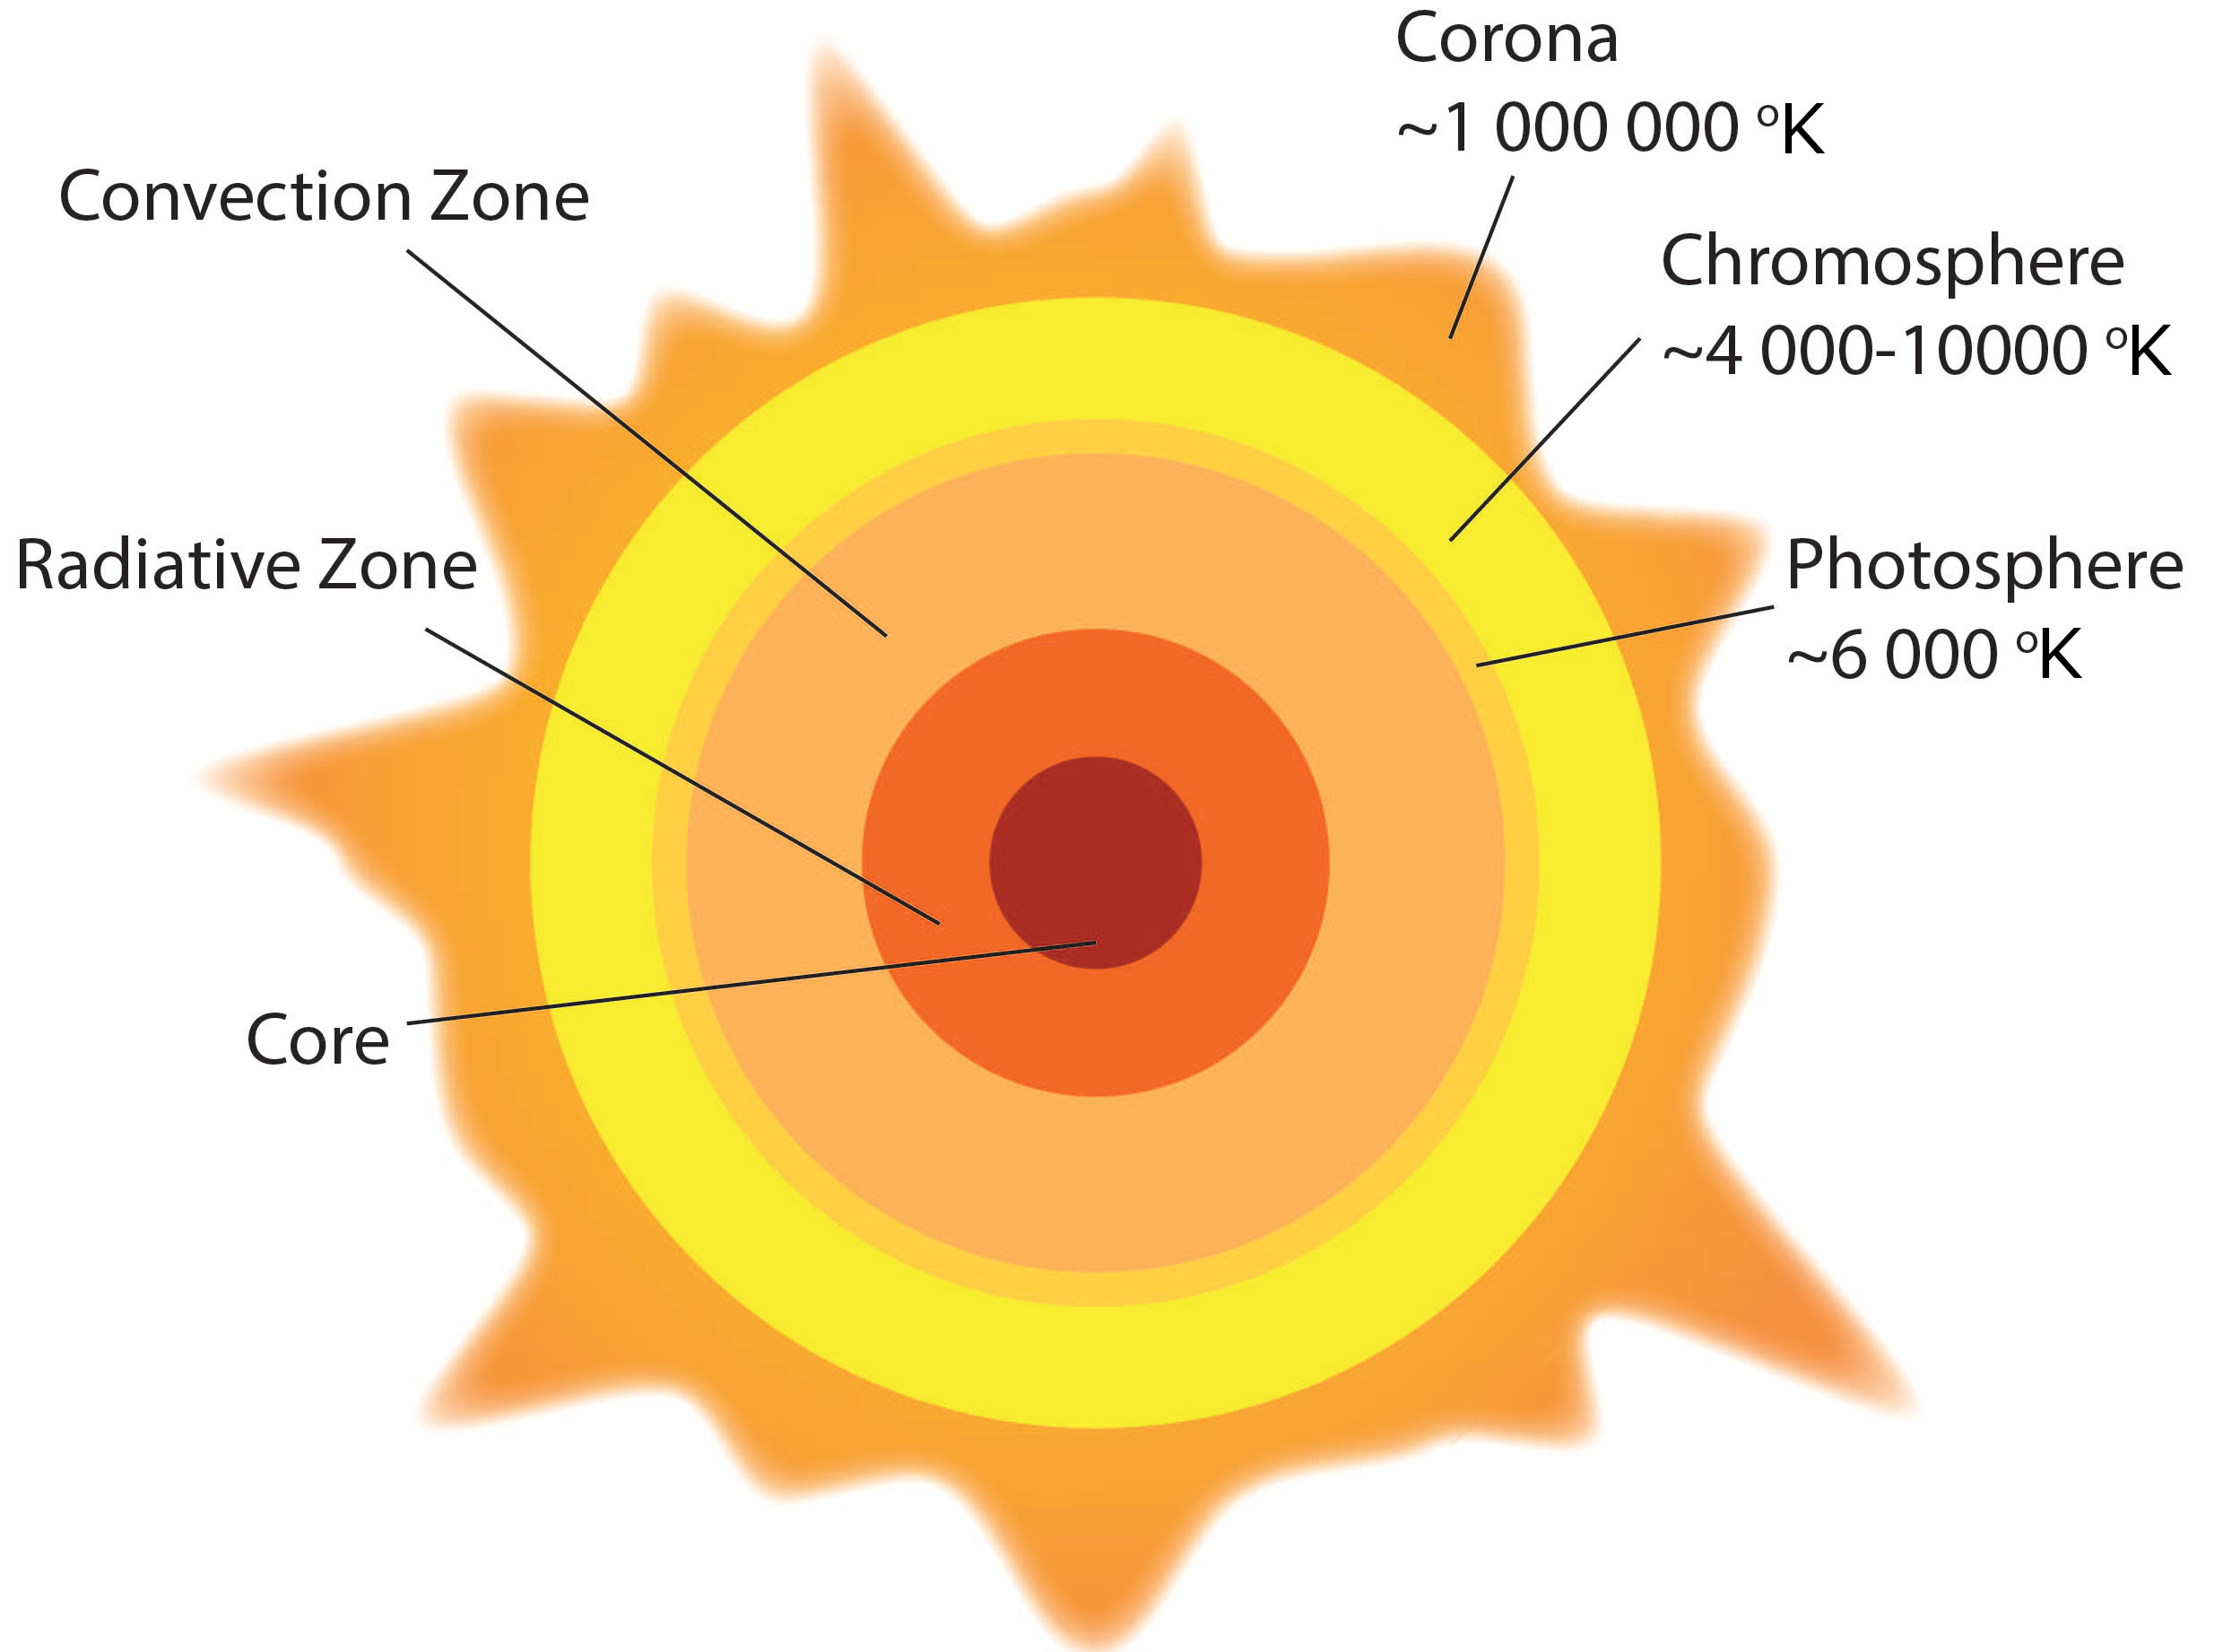
\includegraphics[width=90mm]{images/sun_structure}
%	\url{http://www.phy.cuhk.edu.hk/elearning/Solar_eclipse/Solar_structure.html}
%}



\frame
{
%...................................................................................................
\note<1>[]{when MHD started they could not afford any RT calculations, so they just pre-tabulated cooling rates. Now we can slowly afford some approximate treatment}
%...................................................................................................
	\frametitle{MSc project - Fast approximate non-LTE treatment of the chromosphere}
	\large{\textbf{Current solutions:}}
	\begin{itemize}
		\item Currently used solution: pre-tabulated cooling rates derived from 1D RADYN radiation-hydrodynamic simulations \pause \alert{$\rightarrow$} difficult to expand to more than a handful of elements \\[10pt] \pause
	\end{itemize}
		\large{\textbf{My work:}}
		\begin{itemize}
		\item Escape probability methods \pause \alert{$\rightarrow$} problem with going from 1D to 3D \\[5pt] \pause
		\item Scharmer method: \textit{A new approach to multi-level non-LTE radiative transfer problems, Scharmer's et al (1985)} \\[2pt] 
		    \begin{itemize}
		        \item \large{Eddington Barbier approximation + core saturation approximation}
		    \end{itemize}
	    \end{itemize}
}




\frame
{
%...................................................................................................
\note<1>[]{}
%...................................................................................................
	\frametitle{Conclusions}
	\large{
	\textbf{First project}
	\begin{itemize}
		\item We developed a novel method for fast spectral synthesis. \\%[10pt]
		\item Found optimal sub bins for different wavelength regimes.\\%[10pt]
	    \item Can be tailored for different filters: Strömgren \textit{b} + \textit{y}, Kepler, PLATO  and others.\\%[10pt]
	    \item Significant speed up relative to standard  methods by a factor of at least two orders of magnitude.\\[12pt]
	\end{itemize}
	
	\textbf{Second project}
	\begin{itemize}
		\item Escape probabilities: try the 1.5D approach. 
		\item Scharmer: implement the method into RH 
		\item Compare both methods above to the pre-tabulated cooling rates.\\%[10pt]
	\end{itemize}
	
	}
}

\backupbegin


%%%%%%%%%%%%%%%%%%%%%%%%%%%%%%%%%%%%%%%%%%%%%
%            backup slides                  %
%%%%%%%%%%%%%%%%%%%%%%%%%%%%%%%%%%%%%%%%%%%%%
\frame{
    \frametitle{Backup slides beyond}
    \centering
    \textbf{Here be dragons!}
}


\frame
{
%...................................................................................................
\note<1>[]{}
%...................................................................................................
	\frametitle{Best combinations of 4 sub bins for Str\"omgren \textit{b}}
	\centering
	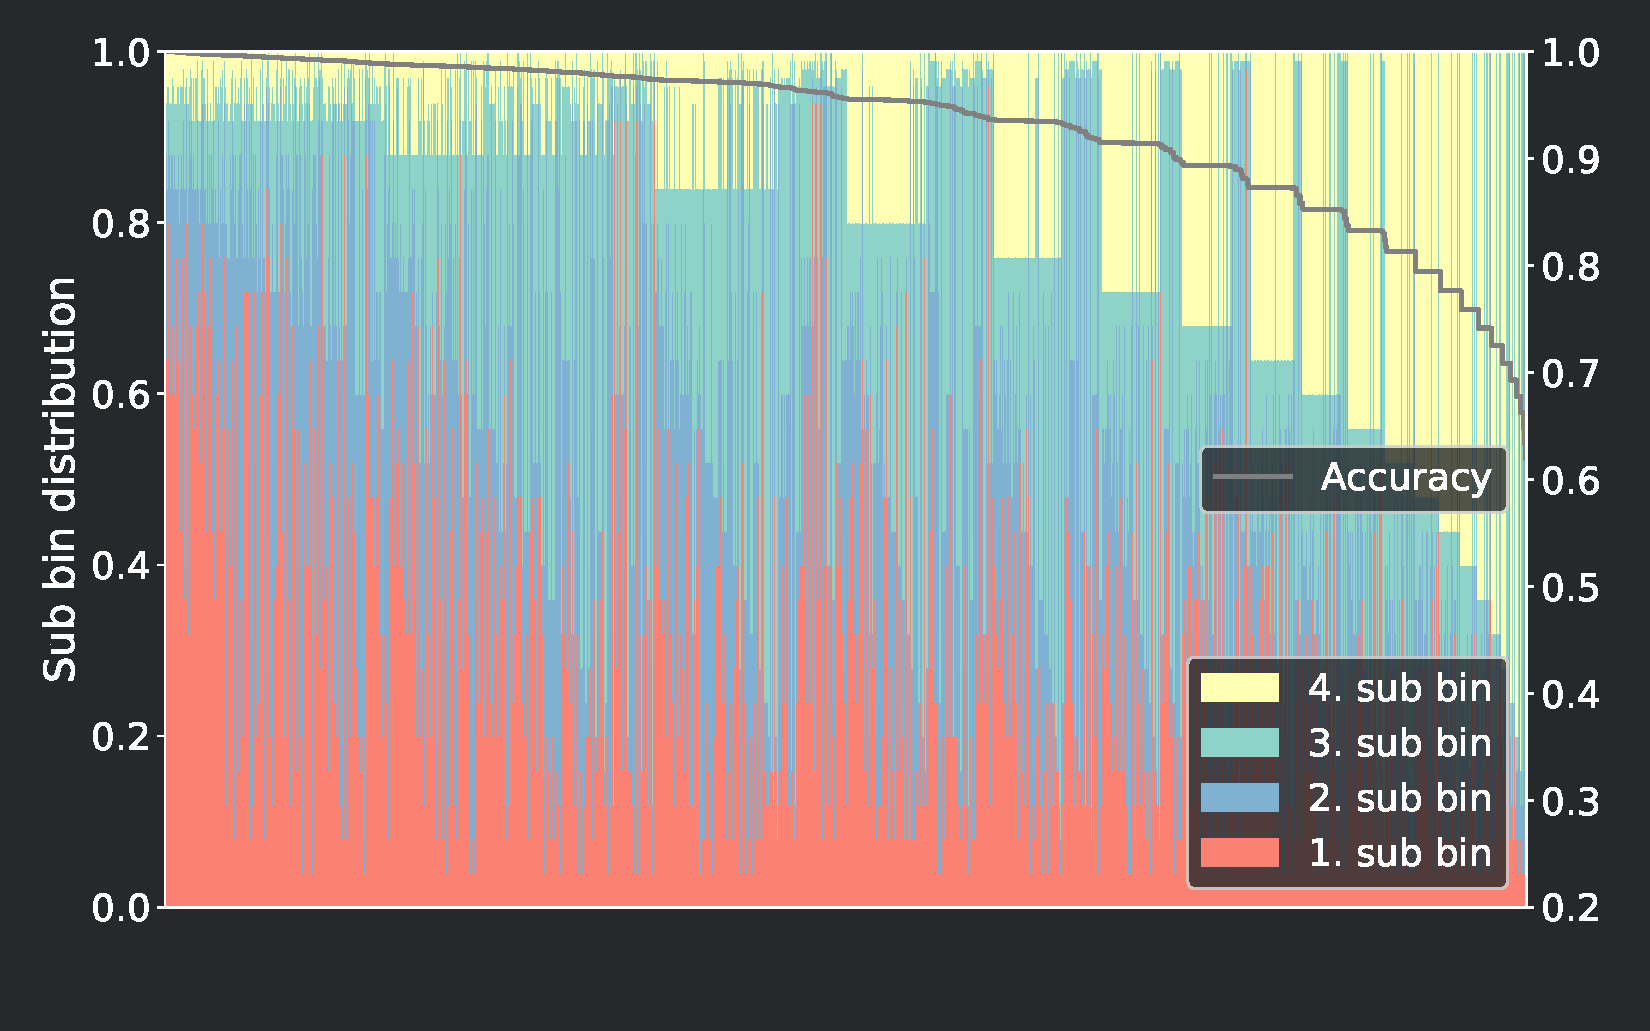
\includegraphics[width=115mm]{images/optimal_stroemgren_0_c_b}
}

\frame
{
%...................................................................................................
\note<1>[]{}
%...................................................................................................
	\frametitle{Formula: value weighted by the derivative}
	\centering
	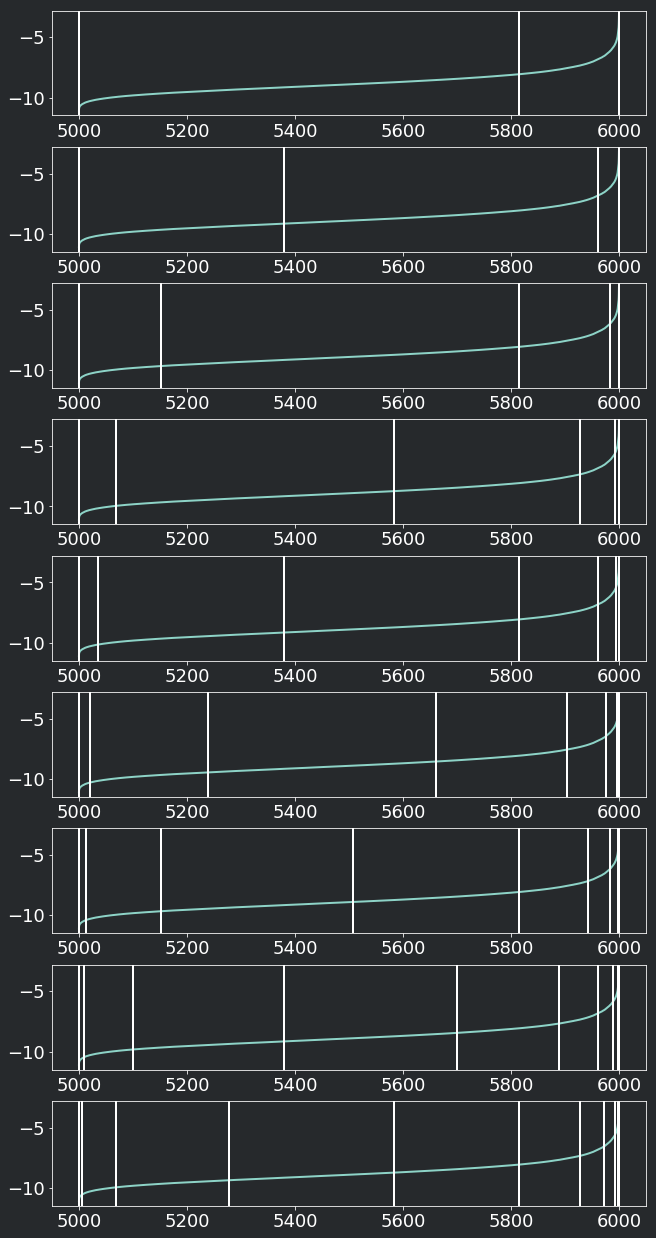
\includegraphics[width=115mm]{images/smart_sub_bins}
}
\frame
{
%...................................................................................................
\note<1>[]{}
%...................................................................................................
	\frametitle{Ascending vs descending sort}
	\centering
	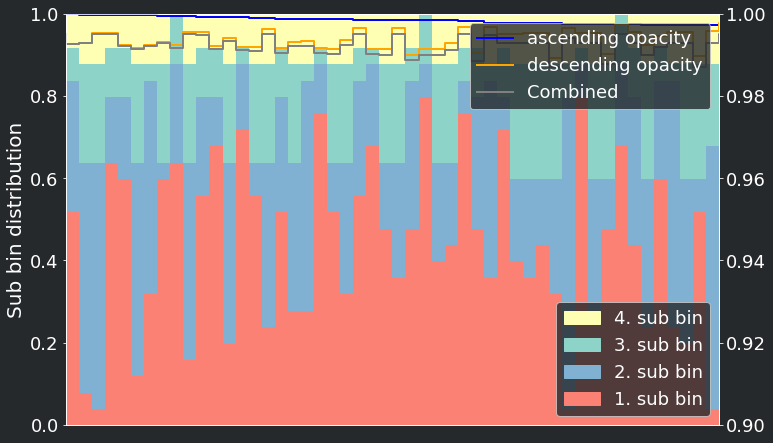
\includegraphics[width=115mm]{images/ascending_descending}
}
\backupend